\begin{table}[!t]
    % \vspace{-0.35cm}
    \caption{Technical Overview of Jetson Platforms}
    % \vspace{-0.3cm}
    \centering
    \begin{tabular}{lcc}
        \Xhline{1pt}
        \textbf{Jetson} & \textbf{AI Performance} & \textbf{GPU Type} \\ 
        \Xhline{0.7pt}
        TX2 & 1.33 TFLOPS & 256-core Pascal \\ \hline
        NX & 21 TOPS & 384-core Volta\\ \hline
        AGX Xavier & 22 TOPS &   512-core Volta \\ \hline
        \Xhline{1pt}
        \textbf{Jetson} & \textbf{CPU Type} & \textbf{ROM} \\ 
        \Xhline{0.7pt}
        TX2 & Denver 2 and ARM 4 & 8 GB LPDDR4\\ \hline
        NX & 6-core Carmel ARM 8 & 8 GB LPDDR4x\\ \hline
        AGX Xavier& 8-core Carmel ARM 8 & 32 GB LPDDR4x \\ \hline
        \Xhline{1pt}
        % \textbf{Jetson}& \textbf{CPU Frequency} & \textbf{GPU Frequency} \\
        % \Xhline{0.7pt}
        % TX2 & 1.2GHz & 0.85Ghz\\ \hline
        % NX & 1.2GHz & 0.8Ghz\\ \hline
        % AGX Xavier& 1.45GHz & 0.9Ghz\\ 
        % \Xhline{1pt}
    \end{tabular}
    \label{jetson-info}
    \vspace{-0.5cm}
\end{table}

\vspace{-0.2cm}
\subsection{Methodology}
\vspace{-0.1cm}
\label{evaluation}
\textbf{Experimental Setup.}
Extensive experiments are conducted on the implemented prototype system with one PS and 80 devices to evaluate the performance of LEGEND.
Specifically, the PS runs on a workstation equipped with an Intel(R) Xeon(R) Platinum 8358P CPU (@ 2.60GHz with 128 cores), 8 NVIDIA RTX A6000 GPUs (48GB memory each) and 512 GB RAM.
In addition, we specify 80 NVIDIA commercial developer kits, including 30 Jetson TX2 kits, 40 Jetson NX kits, and 10 Jetson AGX kits, as devices to construct a heterogeneous system. 
The detailed technical specifications of Jetson TX2, NX, and AGX kits are listed in Table \ref{jetson-info}.

\textbf{Settings of System Heterogeneity.}
To emulate the heterogeneous computing and communication capabilities among devices, we present the following setups.

(1) \textbf{\textit{{For computing.}}}
By specifying different modes of the Jetson devices (\ie, Jetson TX2, NX, and AGX), our prototype system enables these devices to work with varying computing capabilities.
Specifically, Jetson TX2 offers four configurable modes, whereas the Jetson NX and AGX support up to eight modes.
For example, the Jetson AGX with the mode 0 (\ie, the highest performance mode of Jetson AGX) achieves fine-tuning by 100$\times$ faster than the TX2 with the mode 1 (\ie, the lowest performance mode of Jetson TX2).
Besides, to reflect resource varying over time, the devices are configured to randomly change the mode every 20 rounds.

(2) \textbf{\textit{For communication.}}
To replicate the practical network environment, all devices are connected to the PS via Wi-Fi routers in the prototype system.
Concretely, the devices are randomly shuffled and divided into four groups, with each group containing 20 devices. 
Then, these groups are placed at different locations, \ie, 2m, 8m, 14m, and 20m, away from the Wi-Fi routers.
Due to random channel noise and competition among devices, the bandwidth between the PS and devices varies dynamically during the fine-tuning.
The bandwidth of devices is measured by iperf3 \cite{tirumala1999iperf}, which fluctuates between 1Mb/s and 30Mb/s.

\begin{table}[t]
\renewcommand{\arraystretch}{1.1}
    \centering
    \caption{Overview of Datasets for Experimental Evaluation}
    % \vspace{-5px}
    % \resizebox{\textwidth}{!}{
    \begin{tabular}{lccccccc}
         \Xhline{1pt}
         \textbf{Dataset} &  \textbf{Partition Rules} & \makecell{\textbf{\# Training}\\\textbf{Samples}} &\makecell{\textbf{\# Test}\\\textbf{Samples}} \\
         \Xhline{0.7pt}
         SST-2  & non-i.i.d. & 67,349   & 1,821  \\ \hline
         QNLI   & non-i.i.d. & 104,743 & 5,463  \\ \hline
         QQP  & non-i.i.d. & 363,846  & 40,430  \\ \hline
         MNLI  & non-i.i.d. & 392,702  & 9,815  \\ \hline
         GSM-8K   & i.i.d. & 7473 & 1,319  \\ \hline
         MMLU  & i.i.d. & 20,000  & 2,000 \\ \hline
         % Code Generation & Rosetta & 7954 & Prog. Lang. & HumanEvalX & 656 & Llama3.2-1B \\
         % Question Answering & Dolly & 15015 & 8 & Category &  Helm & NA \\
         % Public Dataset & Alpaca & 52002 & \multicolumn{3}{c}{--------------------------------------------------------} & Llama3.2-1B \\
         \Xhline{1pt}
    \end{tabular}
    % }
    \label{tab:datasets}
    \vspace{-0.5cm}
\end{table}


\textbf{Tasks and Models.} 
\rednote{
We evaluate the performance of LEGEND using three representative models downloaded from Hugging Face \cite{wolf2020transformers}, \ie, RoBERTa \cite{liu2019roberta}, DeBERTa \cite{he2021debertav3}, and Llama \cite{touvron2023llama}, across the three categories of tasks, including general language understanding \cite{wang2018glue}, massive multitask understanding \cite{hendrycks2020measuring} and mathematical reasoning \cite{wang2017deep, cobbe2021training}.
}
% \rednote{
% We evaluate the performance of LEGEND with two representative models on two representative NLP tasks, \ie, natural language understanding (NLU) and natural language generation (NLG), .
% } 

\bluenote{
1) \textit{\textbf{General Language Understanding}} aims to assess the natural language understanding capabilities of the models. 
We pick four datasets from the General Language Understanding Evaluation (GLUE) datasets \cite{wang2018glue}, encompassing a diverse spectrum of natural language understanding challenges: SST-2 for sentiment analysis, QNLI for question-based natural language inference, QQP for semantic equivalence, and MNLI for multi-genre textual entailment, respectively.
% , collectively representing critical dimensions of linguistic reasoning and contextual comprehension.
Following the \textit{Dirichlet} distribution with $\alpha = 10$, we build the non-independent and identically (non-i.i.d.) distributed datasets \cite{lin2021fednlp}. 
We fine-tune a 125M-parameter RoBERTa-base model \cite{liu2019roberta} with 12 transformer layers on SST-2 and QNLI, and a 350M-parameter DeBERTa-Large model \cite{he2021debertav3} with 24 transformer layers on QQP and MNLI, respectively.
}

% \rednote{
% 1) \textbf{\textit{Sentiment Analysis}} aims to extract subjective information from text data such as positive, negative, or neutral \cite{medhat2014sentiment}.
% The Stanford Sentiment Treebank (SST-2) dataset \cite{wang2018glue}, which consists of 70,042 sentences (67,349 training samples and 1,821 test samples) from movie reviews with human sentiment annotations, is adopted for sentiment analysis. 
% % We train tailored BERT \cite{devlin2018bert} (with 12 transformer blocks and 110M parameters) for pre-experiments and 
% We train a RoBERTa model \cite{liu2019roberta} with 125M parameters on SST-2.
% RoBERTa is composed of 12 transformer layers, a 768 $\times$ 2 fully-connected hidden layer, and a softmax output layer.
% }
% We train tailored RoBERTa \cite{liu2019roberta} (with 12 transformer blocks and 124M parameters, which is an extension and refinement of BERT \cite{devlin2018bert}) on SST-2.

% \begin{table}
% \footnotesize
%     \caption{Datasets and numbers of samples used in the experiments.}
%     % \vspace{-0.3cm}
%     \centering
%     \resizebox{\linewidth}{!}{
%     \begin{tabular}{|c|c|c|c|}
%     \hline
%     Dataset & Application  & \# Train & \# Test  \\
%     \hline
%     SST-2    & Sentiment Analysis    & 67,349    & 1,821       \\ \hline
%     % MRPC     & Textual similarity      & 3,668     & 408       & F1 score \\
%     QNLI     & Question Answering     & 104,743   & 5,463     \\ \hline
%     % STS-B    & Semantic similarity          & 5,749     & 1,500     & Pearson/Spearman correlation   \\
%     QQP      & Semantic Equivalence & 363,846   & 40,430     \\ \hline
%     MNLI     & Textual Entailment & 392,702   & 9,815     \\ 
%     % RTE      & Textual entailment         & 2,490     & 277       & Accuracy \\
%     % WNLI     & Coreference resolution     & 635       & 71        & Accuracy \\
%     % CoLA     & Linguistic acceptability   & 8,551     & 1,043     & Matthews correlation \\
%     % AGNEWS  & Text classification        & 120,000      & 7,600   & Accuracy \\
%     % 20NEWS  & Text classification       & 11,314        & 7,532   & Accuracy \\
%     \hline
%     \end{tabular}}
%     \label{tab-glue-datasets}
%     \vspace{-0.5cm}
% \end{table}

\begin{figure*}
	\centering
	\subfigure[SST-2]{
		\begin{minipage}[b]{0.23\textwidth}
			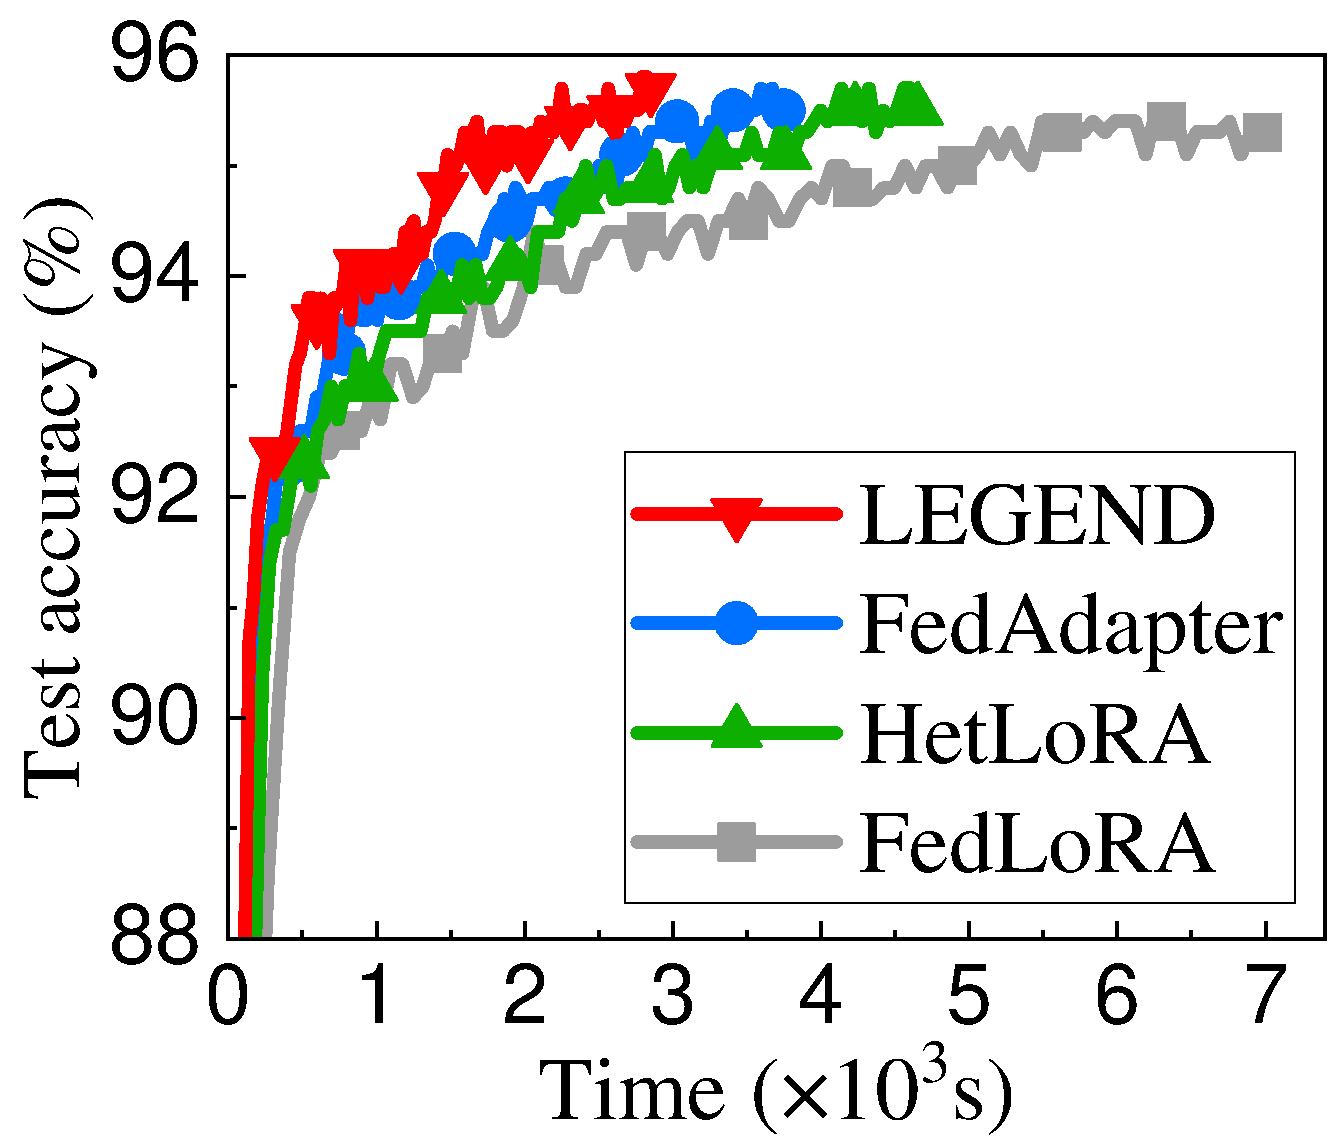
\includegraphics[width=1\textwidth]{figs/final-legend-sst2-time2acc.pdf} 
		\end{minipage}
		\label{roberta-time2acc-sst2}
	}
    	\subfigure[QNLI]{
    		\begin{minipage}[b]{0.23\textwidth}
   		 	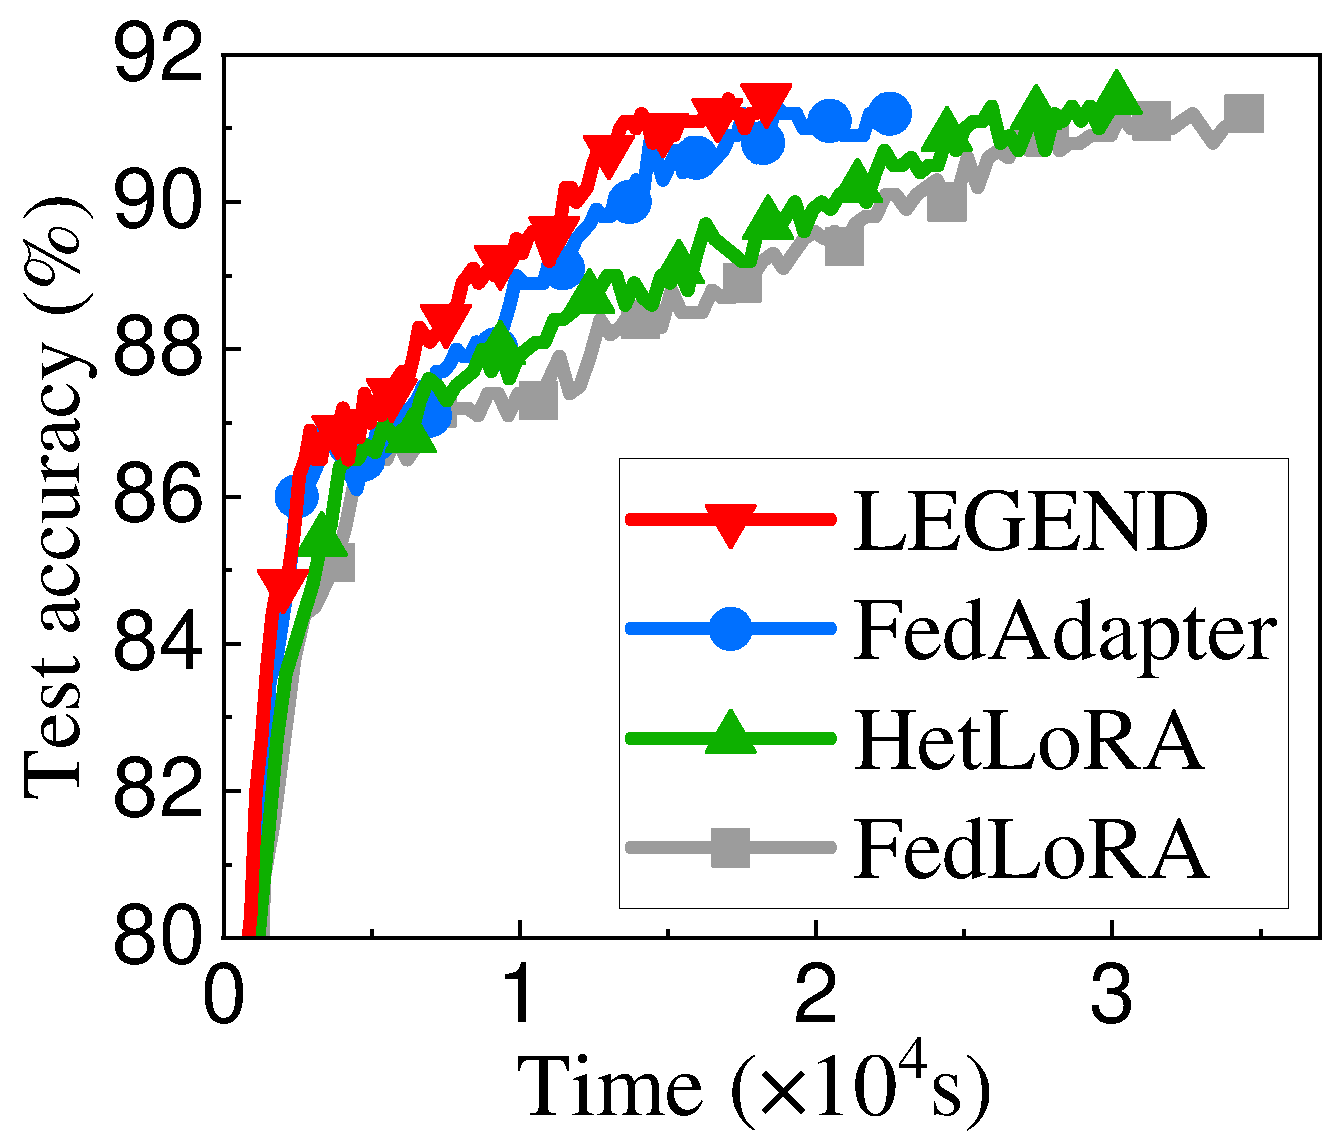
\includegraphics[width=1\textwidth]{figs/final-legend-qnli-time2acc.pdf}
    		\end{minipage}
		\label{roberta-time2acc-qnli}
    	}
	% \\ 
	\subfigure[QQP]{
		\begin{minipage}[b]{0.23\textwidth}
			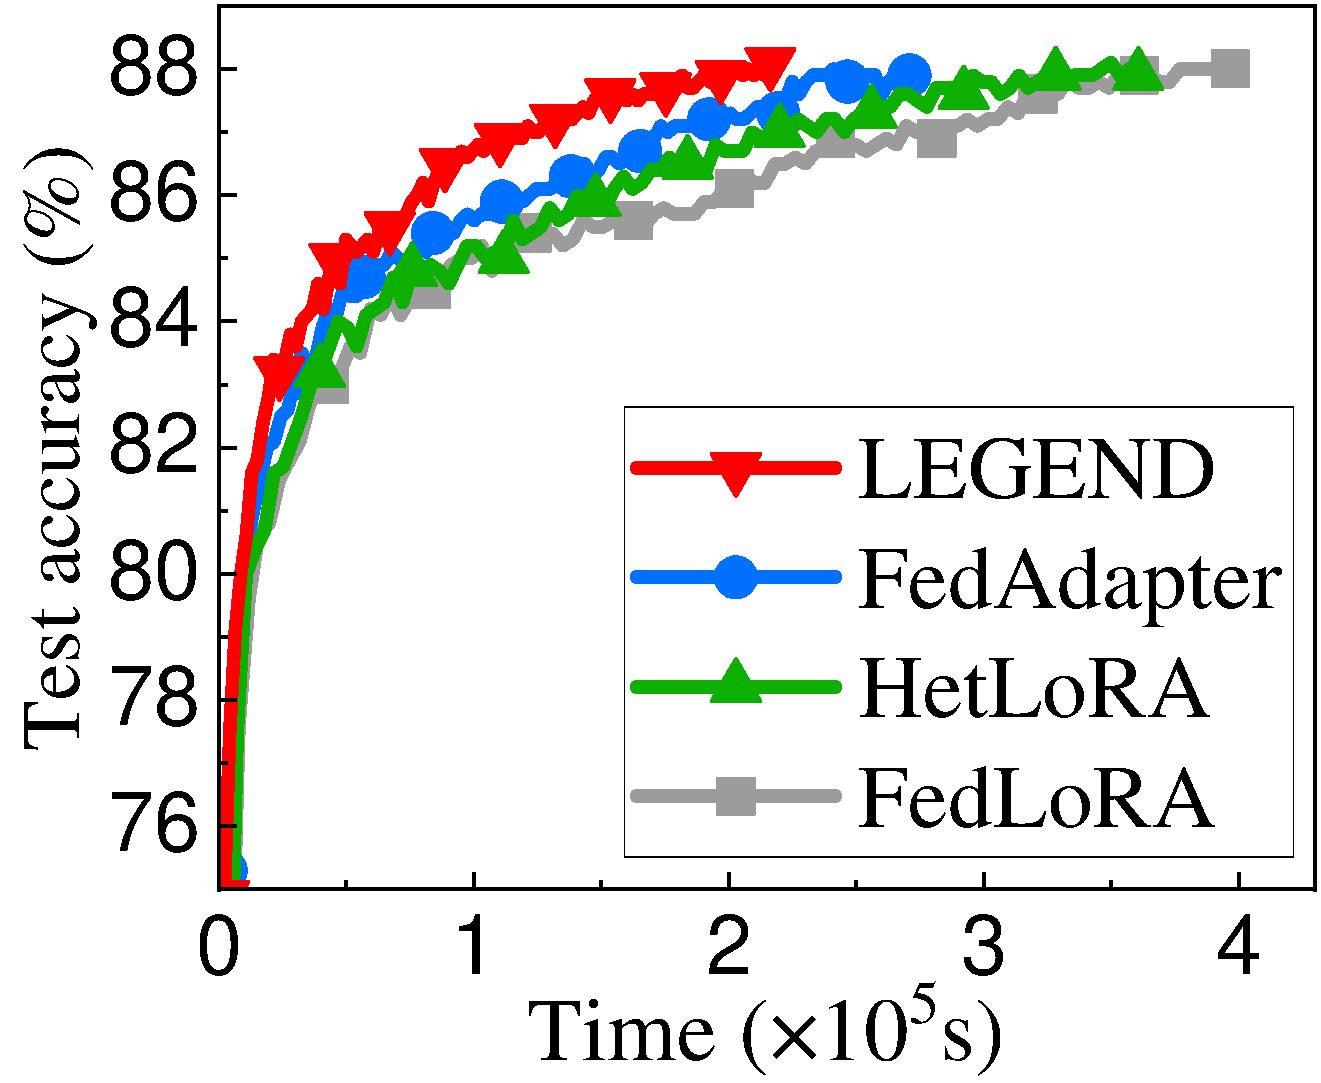
\includegraphics[width=1\textwidth]{figs/final-legend-qqp-time2acc.pdf} 
		\end{minipage}
		\label{deberta-time2acc-qqp}
	}
    	\subfigure[MNLI]{
    		\begin{minipage}[b]{0.23\textwidth}
		 	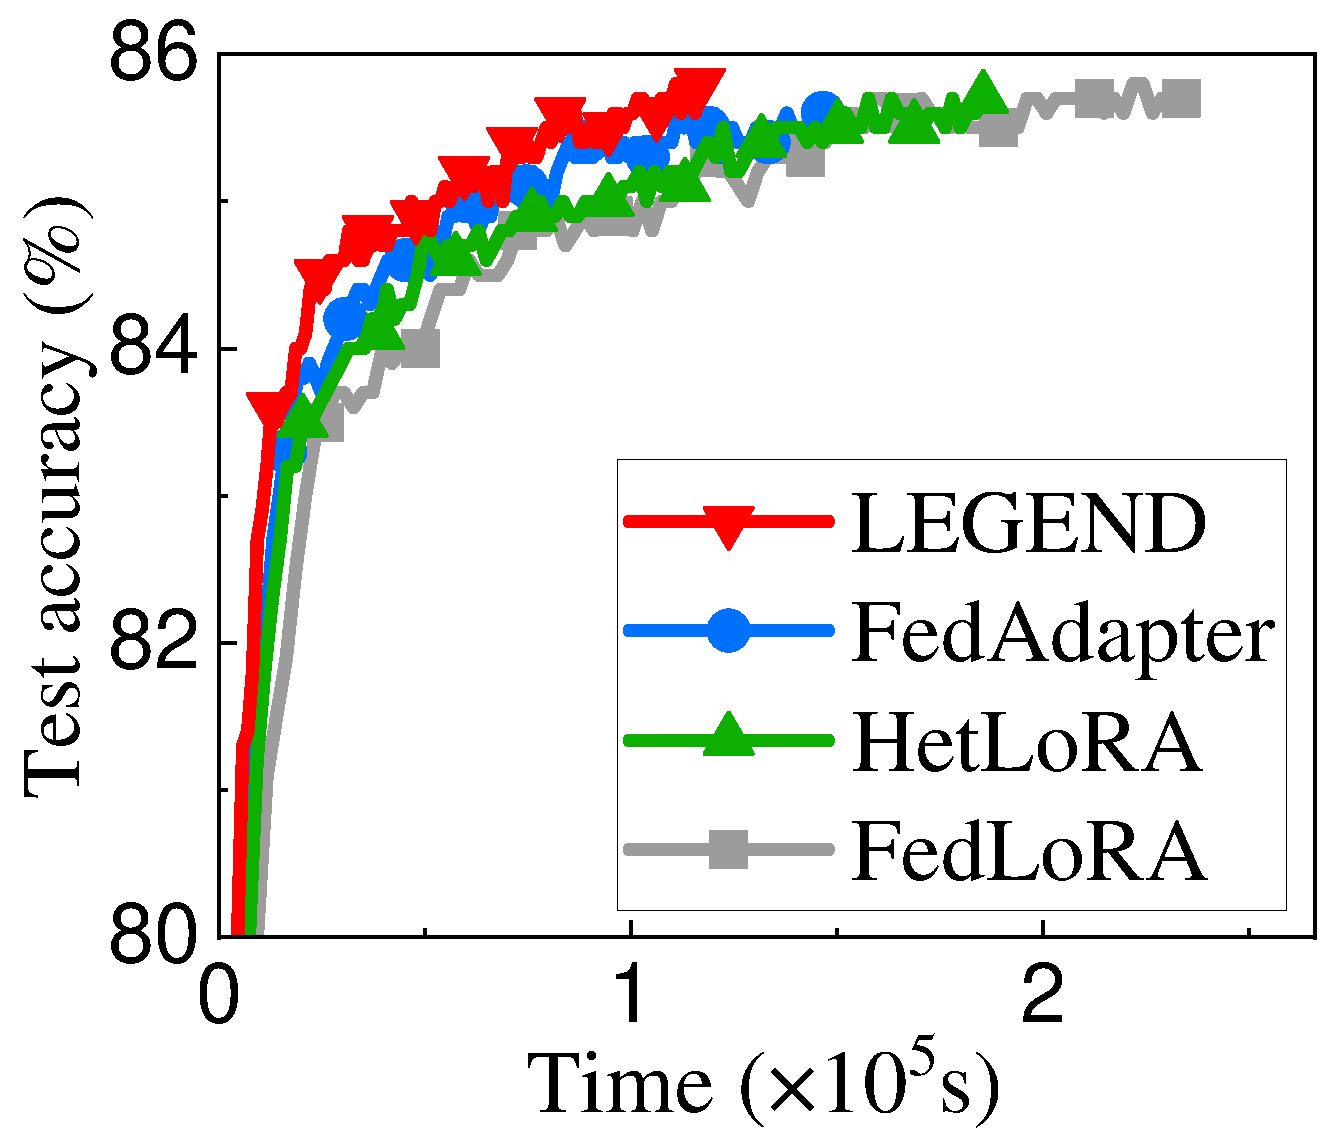
\includegraphics[width=1\textwidth]{figs/final-legend-mnli-time2acc.pdf}
    		\end{minipage}
		\label{deberta-time2acc-mnli}
    	}
        \vspace{-0.3cm}
	\caption{Fine-tuning process of four approaches on general language understanding tasks.}
        \vspace{-0.4cm}
        \label{time-acc}
\end{figure*}

\begin{figure*}
	\centering
    % \hspace{3.5mm}
	\subfigure[Time to reach 95\% accuracy]{
		\begin{minipage}[b]{0.23\textwidth}
			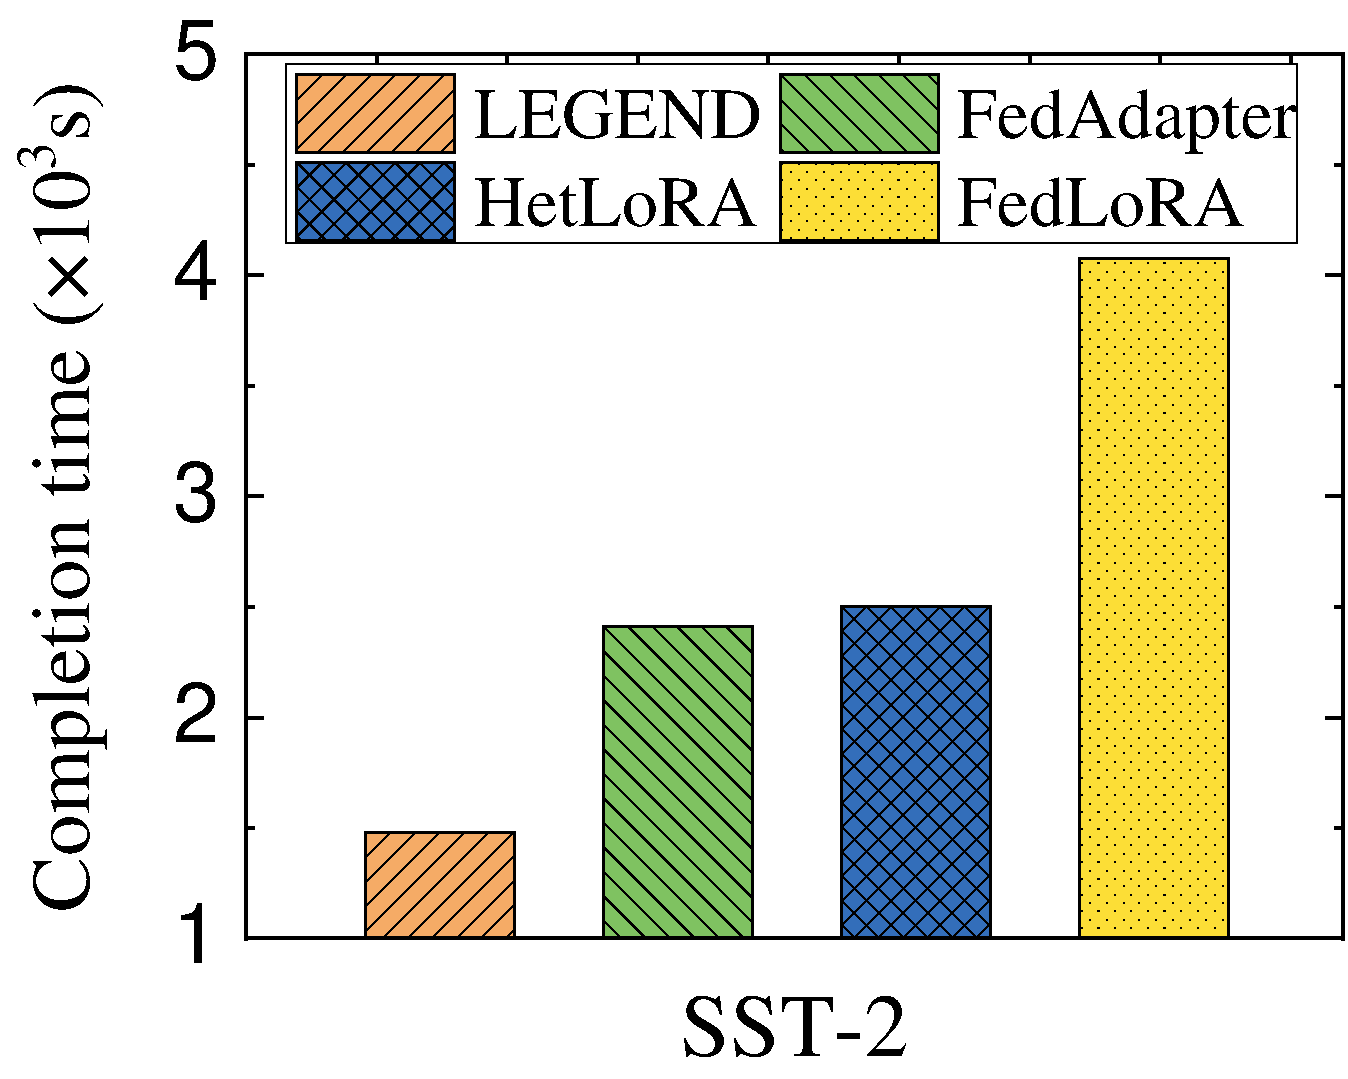
\includegraphics[width=1\textwidth]{figs/completion-time-sst2.pdf} 
		\end{minipage}
		\label{roberta-completion-sst2}
	}
    	\subfigure[Time to reach 90\% accuracy]{
    		\begin{minipage}[b]{0.23\textwidth}
   		 	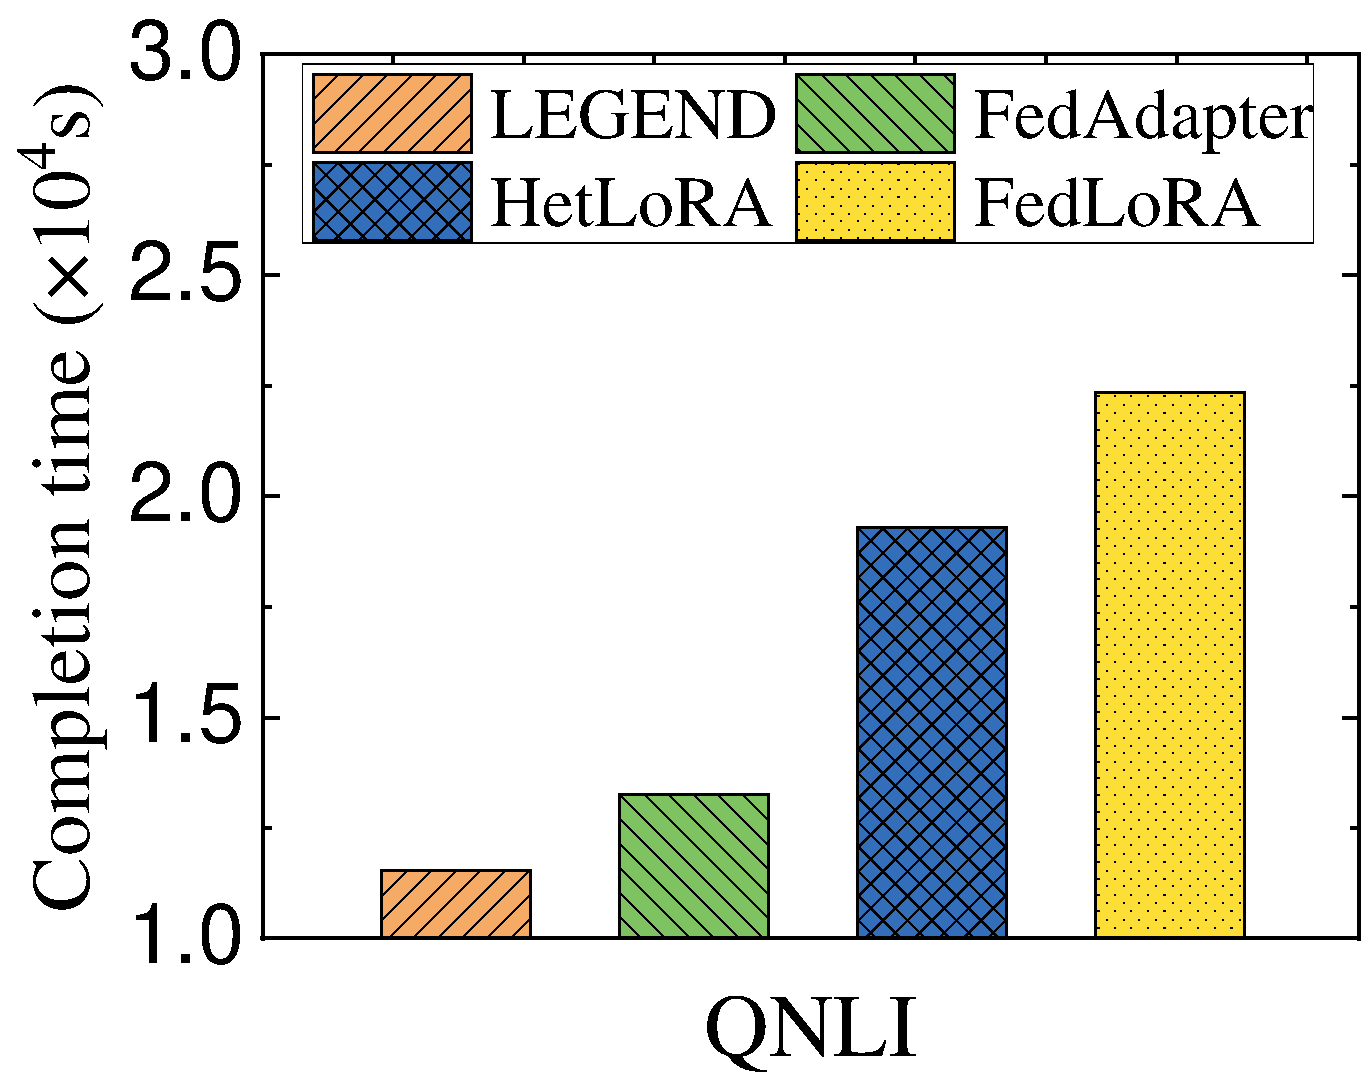
\includegraphics[width=1\textwidth]{figs/completion-time-qnli.pdf}
    		\end{minipage}
		\label{roberta-completion-qnli}
    	}
	% \\ 
	\subfigure[Time to reach 87\% accuracy]{
		\begin{minipage}[b]{0.23\textwidth}
			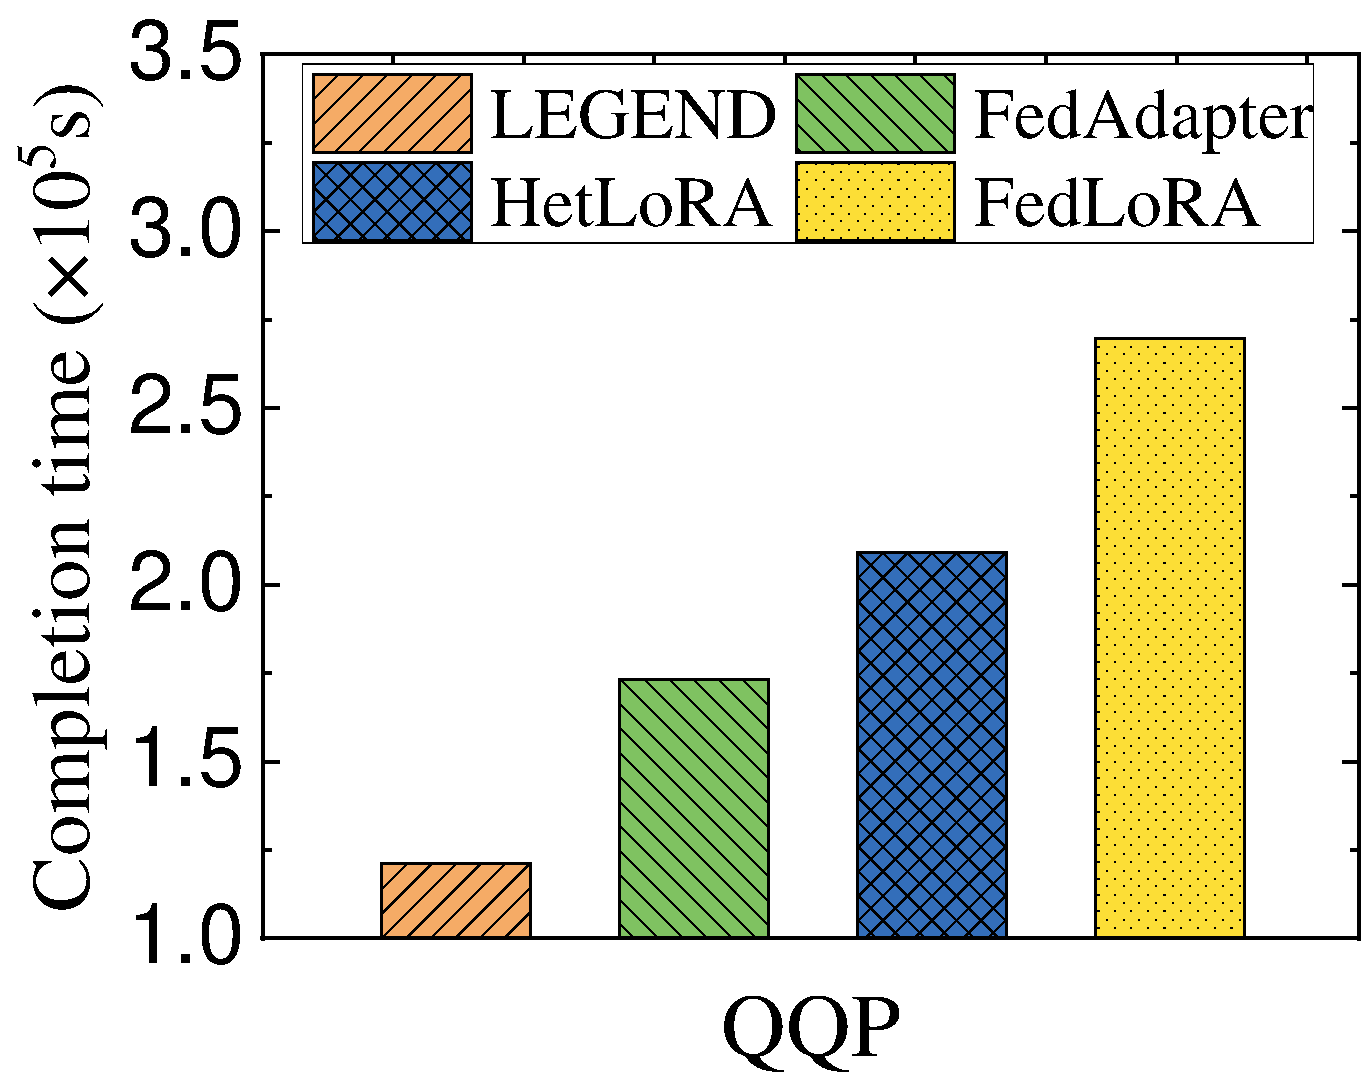
\includegraphics[width=1\textwidth]{figs/completion-time-qqp.pdf} 
		\end{minipage}
		\label{deberta-completion-qqp}
	}
    	\subfigure[Time to reach 85\% accuracy)]{
    		\begin{minipage}[b]{0.23\textwidth}
		 	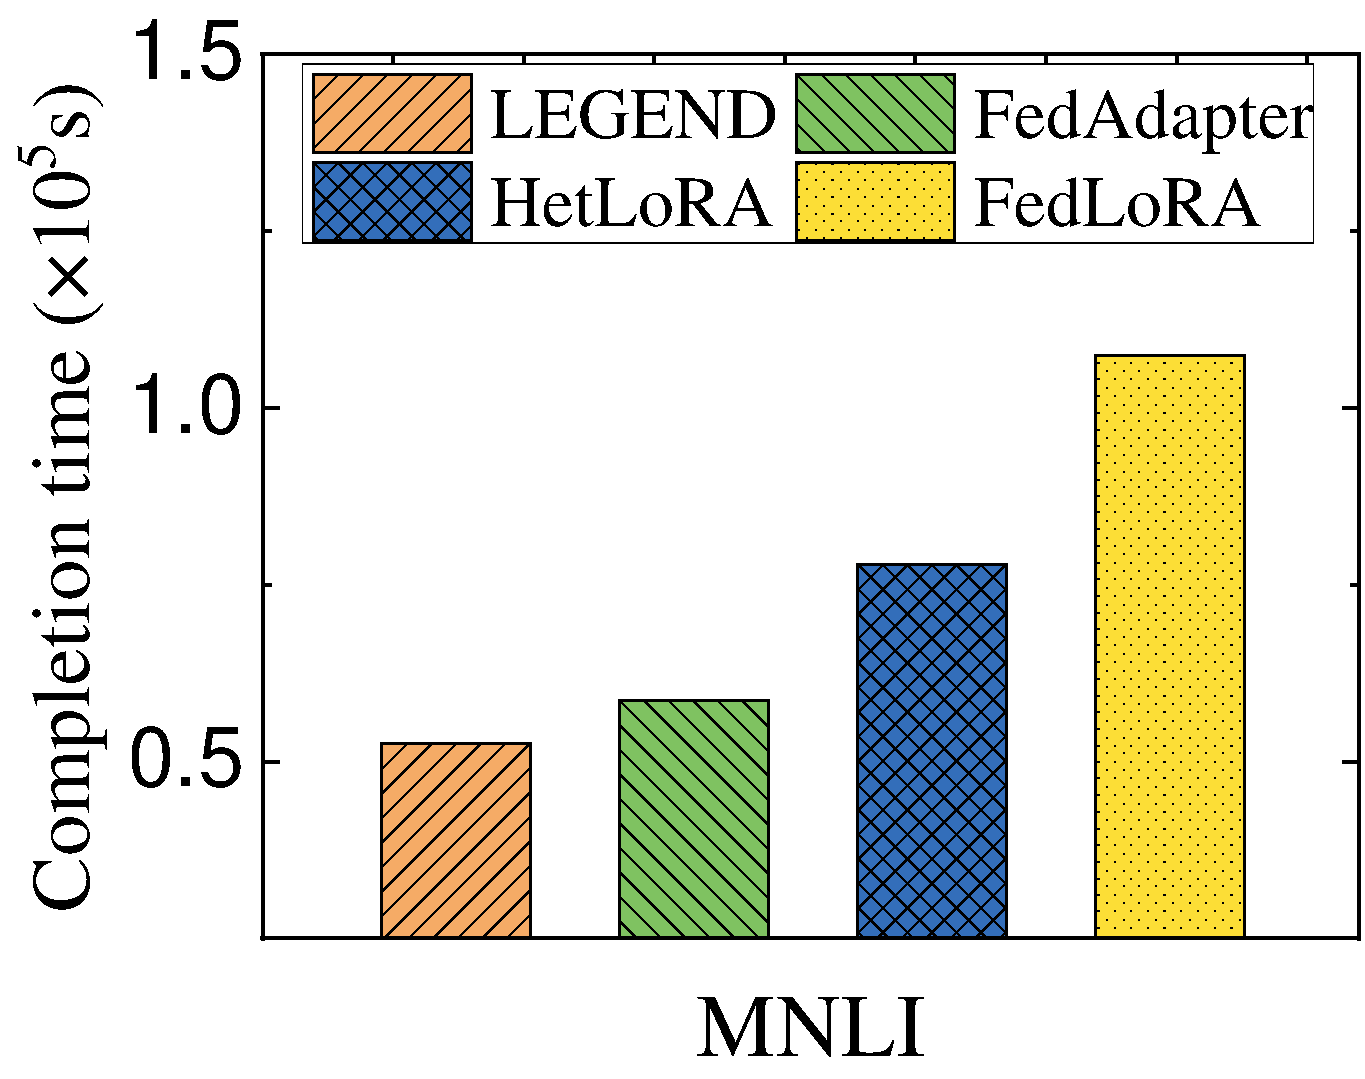
\includegraphics[width=1\textwidth]{figs/completion-time-mnli.pdf}
    		\end{minipage}
		\label{deberta-completion-mnli}
    	}
        \vspace{-0.3cm}
	\caption{Completion time of four approaches on general language understanding tasks.}
        \vspace{-0.4cm}
        \label{completion-time}
\end{figure*}

\begin{figure}[t]
    \hspace{10mm}
    \centering
    \subfigure[{Fine-tuning process (MMLU)}]{
        \hspace{0.7mm}
        \begin{minipage}[b]{0.5\linewidth}
        \centering
        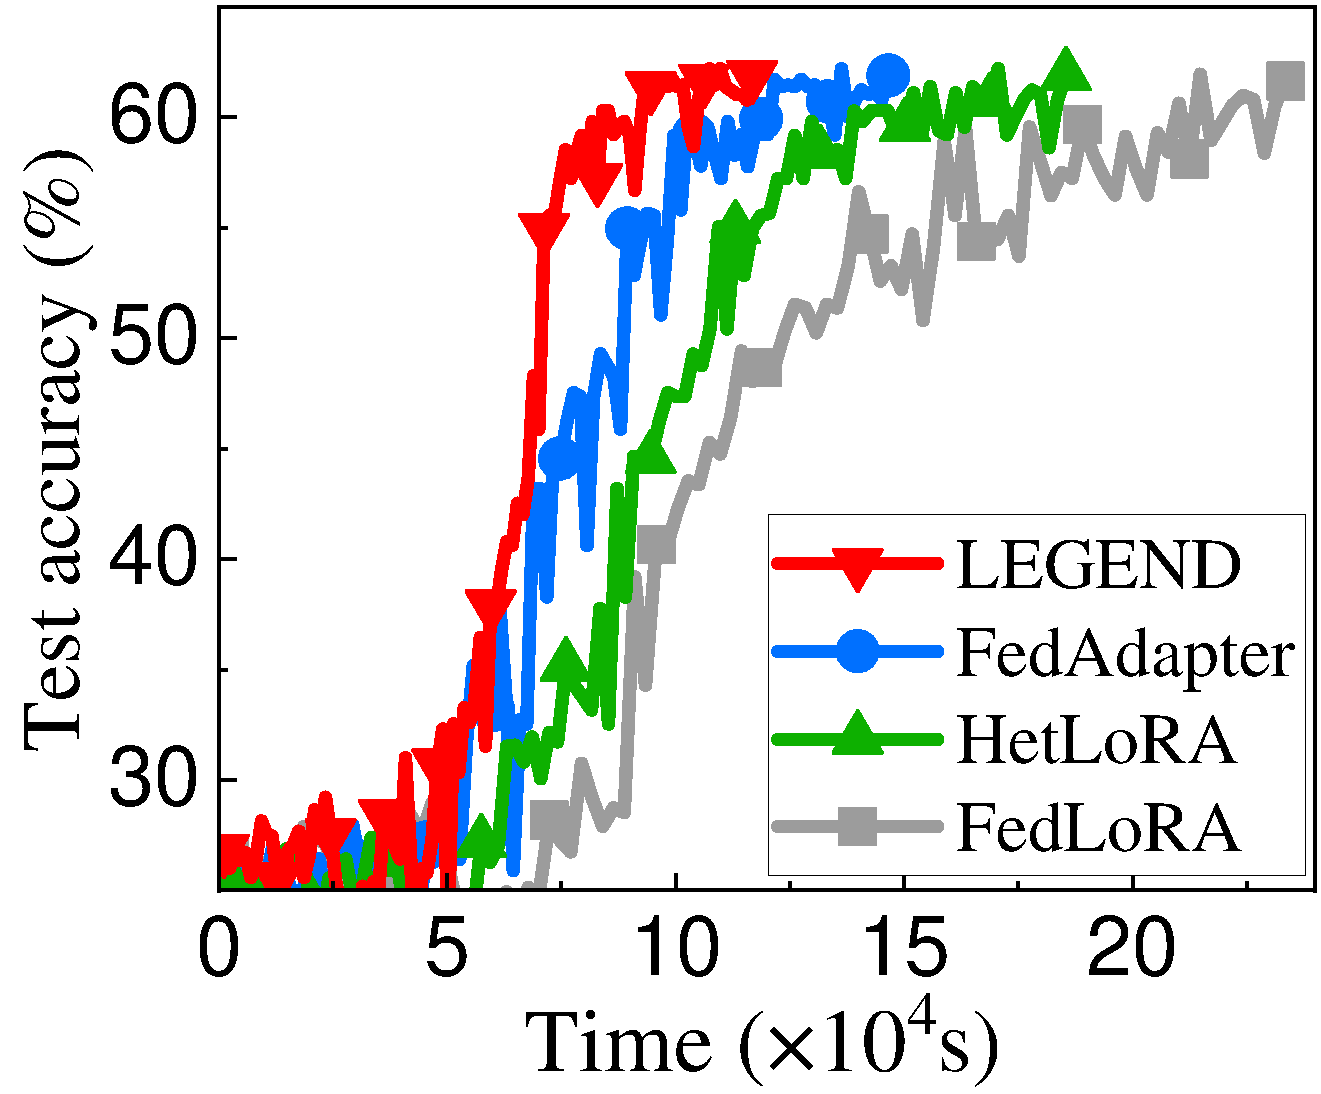
\includegraphics[width=1.6in]{figs/llama2-7b-mmlu.pdf}
        \end{minipage}%
        \label{llama2-7b-mmlu-time2acc}
    }%
    \subfigure[{Time to reach 60\% accuracy}]{
        \begin{minipage}[b]{0.5\linewidth}
        \centering
        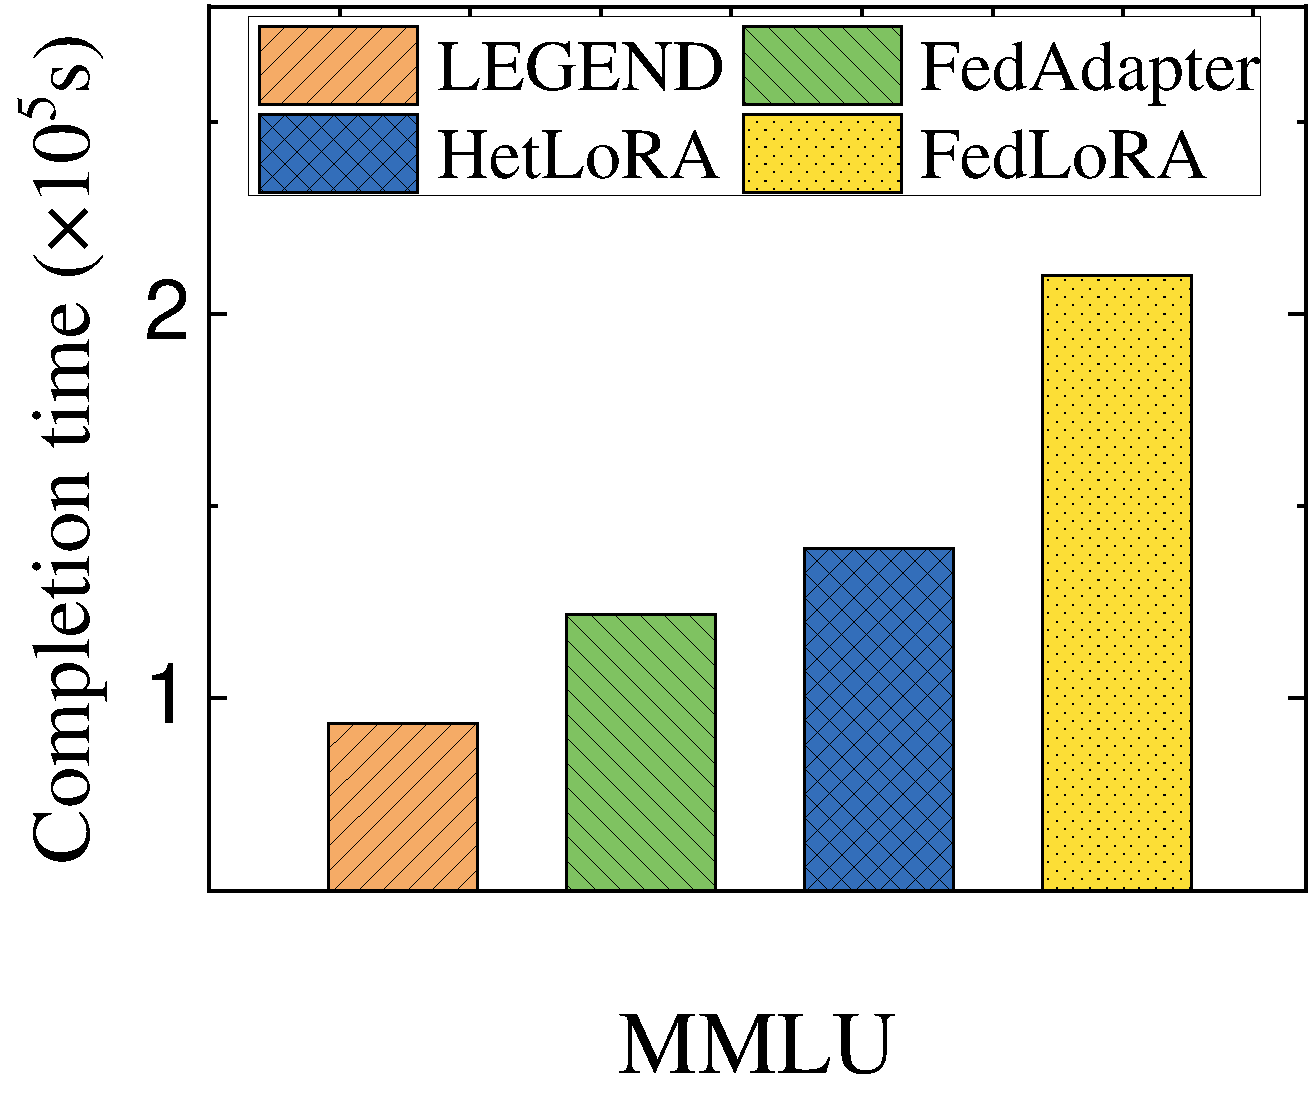
\includegraphics[width=1.6in]{figs/completion-time-mmlu.pdf}
        \end{minipage}%
        \label{llama2-7b-mmlu-completion}
    }%
    \centering
    \vspace{-0.5cm}
    \caption{\bluenote{Results on massive multitask understanding tasks.}}
    \label{mmlu-results}
    \vspace{-0.6cm}
\end{figure}



% 2) \textbf{\textit{Question Answering.}}
% \rednote{
% 2) \textbf{\textit{Question Answering}} focuses on generating concise and accurate answers to questions of natural language by comprehending the query and retrieving relevant information from data sources \cite{rajpurkar2016squad}.
% We utilize the Question-answering Natural Language Inference (QNLI) dataset \cite{wang2018glue}, a classification dataset consisting of question-sentence pairs in the corresponding context, for this application. 
% The dataset includes 104,743 and 5,463 samples for training and test, respectively.
% The model employed on QNLI is the same as that on SST-2.
% }
% The objective of the dataset is to determine whether the context sentence contains the answer to the question.
% A tailored RoBERTa is trained on this dataset.


% \rednote{
% 3) \textbf{\textit{Semantic Equivalence}} determines whether two given texts convey the same meaning or not, disregarding differences in word choice or syntax \cite{chandrasekaran2021evolution}. 
% We use the Quora Question Paris (QQP) dataset \cite{wang2018glue} for evaluation.
% The QQP dataset is a collection of question pairs composed of 363,846 and 40,430 samples for training and test, respectively, from the website Quora. 
% DeBERTa-Large \cite{he2021debertav3} with 430M parameters is trained on QQP, consisting of 24 transformer layers, a 768 $\times$ 2 fully-connected layer, and a softmax output layer.}
% We train a customized DeBERTa-Large model \cite{he2021debertav3} on QQP, which is the latest version of the DeBERTa model series. 
% The DeBERTa-Large contconsisting of 24 transformer layers


% \rednote{
% 4) \textbf{\textit{Textual Entailment}} reasons the logical relationship between a given premise and a corresponding hypothesis, which can be classified as entailment, contradiction, or neutral \cite{ghuge2014survey}. 
% The Multi-Genre Natural Language Inference (MNLI) dataset \cite{wang2018glue}, a crowdsourced collection of sentence pairs with textual entailment annotations, is adopted for textual entailment.
% The dataset consists of 392,702 and 9,815 samples for training and test, respectively.
% % The objective of this task is to determine the logical relationship between a given premise and a corresponding hypothesis, which can be classified as entailment, contradiction, or neutral. 
% We train a tailed DeBERTa-Large, which is composed of 24 transformer layers, a 768 $\times$ 3 fully-connected layer, and a softmax output layer.
% }

\bluenote{
2) \textbf{\textit{Massive Multitask Understanding}} 
aims to test model generalization and knowledge transfer by fine-tuning across multiple related tasks. 
We utilize the Massive Multitask Language Understanding (MMLU) datasets \cite{hendrycks2020measuring} for the evaluation, which is a comprehensive multiple-choice benchmark spanning 57 tasks across diverse academic domains. 
By sampling 20,000 training and 2,000 test samples from the \textit{auxiliary\_train} subset, we create a dataset that challenges models to demonstrate broad knowledge and nuanced reasoning capabilities.
We fine-tune a 7B-parameter Llama2 model (\ie, Llama2-7B) \cite{touvron2023llama}, which is composed of 32 transformer layers, on this customized dataset.
}

\bluenote{
3) \textbf{\textit{Mathematical Reasoning}}
serves as a critical task for evaluating the models' logical reasoning and computational reasoning capabilities. 
We employ the Grade School Math (GSM-8K) dataset \cite{cobbe2021training}, which is a widely recognized benchmark designed to evaluate models' elementary mathematical reasoning and problem-solving abilities. 
It comprises 7,473 training and 1,319 test problems, each requiring multi-step reasoning and arithmetic calculations, reflecting the complexity of grade-school mathematics. 
This dataset challenges models to demonstrate logical consistency, numerical computation, and interpretive skills essential for advanced mathematical understanding.
We fine-tune Llama2-7B on this dataset.
}

% \begin{table}
%     \caption{Datasets used in the experiments}
%     \centering
%     \resizebox{\linewidth}{!}{
%     \begin{tabular}{|c|c|c|c|c|}
%     \hline
%     Dataset & Application  & \# Train & \# Test & Model \\
%     \hline
%     SST-2    & Sentiment Analysis    & 67,349    & 1,821       & RoBERTa  \\ \hline
%     % MRPC     & Textual similarity      & 3,668     & 408       & F1 score \\
%     QNLI     & Question Answering     & 104,743   & 5,463     & RoBERTa \\ \hline
%     % STS-B    & Semantic similarity          & 5,749     & 1,500     & Pearson/Spearman correlation   \\
%     QQP      & Semantic Equivalence & 363,846   & 40,430    & DeBERTa-Large \\ \hline
%     MNLI     & Textual Entailment & 392,702   & 9,815     & DeBERTa-Large \\ 
%     % RTE      & Textual entailment         & 2,490     & 277       & Accuracy \\
%     % WNLI     & Coreference resolution     & 635       & 71        & Accuracy \\
%     % CoLA     & Linguistic acceptability   & 8,551     & 1,043     & Matthews correlation \\
%     % AGNEWS  & Text classification        & 120,000      & 7,600   & Accuracy \\
%     % 20NEWS  & Text classification       & 11,314        & 7,532   & Accuracy \\
%     \hline
%     \end{tabular}}
%     \label{tab-glue-datasets}
% \end{table}




\textbf{Baselines.}
To evaluate the effectiveness of LEGEND, we adopt two LoRA-based approaches (\ie, naive FedLoRA \cite{zhang2023fedpetuning} and advanced HetLoRA \cite{cho2023heterogeneous}) and the state-of-the-art FedFT approaches (\ie, FedAdapter \cite{cai2022fedadapter}) as baselines.

1) \textbf{FedLoRA} 
integrates LoRA \cite{hu2021lora} into FedFT, where all the devices fine-tune the same local model with the identical rank applied to all transformer layers.

2) \textbf{HetLoRA}  
is an advanced LoRA-based approach for FedFT, which assigns each device with a diverse but appropriate LoRA rank for fine-tuning all transformer layers of its local model so as to deal with system heterogeneity.

3) \textbf{FedAdapter} 
is the state-of-the-art FedFT approach, which introduces Adapters \cite{houlsby2019parameter} in FedFT and dynamically searches for the optimal Adapter configuration to improve fine-tuning efficiency.


\textbf{Metrics.}
The following metrics are adopted to evaluate the performance of LEGEND and the baselines.

1) \textbf{\textit{Test Accuracy}} reflects the accuracy of the models fine-tuned by different approaches on the test datasets, measured by the proportion of correctly predicted data.
Specifically, we record the test accuracy of the global model (the model after aggregation at the PS) in each round.

2) \textit{\textbf{Completion time}} represents the total wall-clock time required for fine-tuning a model to achieve a target accuracy. 
For fair comparisons, we set the target accuracy as the minimum accuracy achieved by the four methods. 
We record the time of each round, summing it up to obtain the completion time, and also record the average waiting time to reflect the fine-tuning efficiency of different approaches.

3) \textit{\textbf{Communication Traffic}} is recorded by summing up the traffic for transmitting the trainable parameters between the PS and devices during model fine-tuning, which is used to measure the communication efficiency of each approach.

\textbf{Experimental Parameters.}
\bluenote{
By default, all experiments are carried out on our prototype system and run 100 rounds.
Each device fine-tunes 1 epoch per round using AdamW \cite{loshchilov2017decoupled} optimizer locally.
The learning rate is set as 0.002 and decays according to a cosine scheduler.
The batch size is fixed at 4 and the maximum sequence length is set to 512 for all experiments.
}
\vspace{-0.2cm}
% We adopt gradient accumulation \cite{} to alleviate the on-device memory constraint.
% For SST-2, the batch size is 16 and the gradient accumulation step is specified as 2.
% The batch size and the gradient accumulation step for QNLI, QQP, and MNLI are identical and are set as 4 and 4, respectively \cite{}.

% For SST-2, the batch size is set as 16 and the maximum sequence length of the input text is specified as 256. 
% The batch size and max sequence length for QNLI, QQP, and MNLI are identical, which are set as 4 and 512, respectively.
% \rednote{For decoder-only model}
% The batch size is set as 16 for SST-2, 4 for QNLI, QQP, and MNLI.
% max sequence length of the input text as 256 for SST-2, 512 for QNLI, QQP, and MNLI. 
% Followed by previous works \cite{lin2021fednlp, cai2022fedadapter, zhang2023fedpetuning}, the local training epoch is set to 1. 
% The rank of FedLoRA is set to 16, the ranks of HetLoRA are set within $\{ 2, 4, 8, 16, 32 \}$, and the rank budget of LEGEND is set equal to FedLoRA.
% \vspace{-0.2cm}

\subsection{Overall Performance}
\vspace{-0.1cm}
% \rednote{\textbf{Accuracy improved; Acceleration; Communication Cost; Waiting time}}
% \textbf{Accelerating the training process.}
% \textbf{Convergence Performance.}
Firstly, we conduct sets of experiments to evaluate the performance of LEGEND and the baselines.
The fine-tuning processes and the completion time of the general language understanding task are presented in Figures \ref{time-acc} and \ref{completion-time}, respectively.
% \rednote{The completion time} of different approaches upon achieving the target accuracy is shown in Figure .
By the results, LEGEND achieves the fastest convergence rate, outperforming the other approaches by a significant margin on all tasks. 
By assigning smaller LoRA depths with an optimized rank distribution for resource-constrained devices, LEGEND effectively enhances fine-tuning performance while reducing the time for local fine-tuning.
% Simultaneously, LEGEND adapts a suitable LoRA rank distribution to ensure the model performance further.
For instance, by Figures \ref{roberta-time2acc-sst2} and \ref{roberta-completion-sst2}, LEGEND takes only 1,479s to achieve 85\% accuracy on SST-2, while FedAdapter, HetLoRA, and FedLoRA take 2,412s, 2,503s, and 4,074s, respectively.
Compared to FedAdapter, HetLoRA, and FedLoRA, LEGEND provides 1.6$\times$, 1.7$\times$, and 2.8$\times$ speedup, respectively. 
By Figures \ref{roberta-time2acc-qnli} and \ref{roberta-completion-qnli}, LEGEND also outperforms the other baselines in terms of completion time for QNLI. 
Similarly, Figures \ref{deberta-time2acc-qqp} and \ref{deberta-completion-qqp} show that LEGEND takes 121,156s to achieve 87\% accuracy for QQP, while FedAdapter, HetLoRA, and FedLoRA consume 173,375s, 209,196s, and 269,749s, respectively. 
LEGEND separately achieves a speedup of 1.4$\times$, 1.7$\times$, and 2.2$\times$, compared with FedAdapter, HetLoRA, and FedLoRA.
% HetLoRA has the slowest convergence rate because it uses different rank local models to deal with resource constraints and system heterogeneity problems, but the rank has little impact on the overhead of computing resources, which is not enough to balance the gap in computing power between different devices, and aggregating different models leads to inefficiency and poor model performance.
For MNLI, as shown in Figures \ref{deberta-time2acc-mnli} and \ref{deberta-completion-mnli}, LEGEND speeds up the fine-tuning process by about 1.2$\times$, 1.5$\times$, and 2.1$\times$, compared to FedAdapter, HetLoRA, and FedLoRA, respectively. 
\bluenote{
Then, we present the experimental results for massive multitask understanding and mathematical reasoning tasks in Figures \ref{mmlu-results} and \ref{gsm8k-results}.
LEGEND consistently outperforms all other baselines, significantly accelerating the fine-tuning process. 
Specifically, as shown in Figure \ref{mmlu-results}, LEGEND achieves a speedup of 1.3$\times$, 1.5$\times$, and 2.3$\times$ compared to FedAdapter, HetLoRA, and FedLoRA, respectively. 
In Figure \ref{gsm8k-results}, LEGEND reduces the total completion time required to achieve 30\% accuracy by approximately 26\%, 41\%, and 54\% when compared to FedAdapter, HetLoRA, and FedLoRA, respectively.
These results demonstrate the superiority of LEGEND in accelerating the fine-tuning process through joint optimization of LoRA depth and rank distribution.
}

\begin{figure}[t]
    \hspace{-6mm}
    \centering
    \subfigure[Fine-tuning process (GSM-8K)]{
        \begin{minipage}[b]{0.5\linewidth}
        \centering
        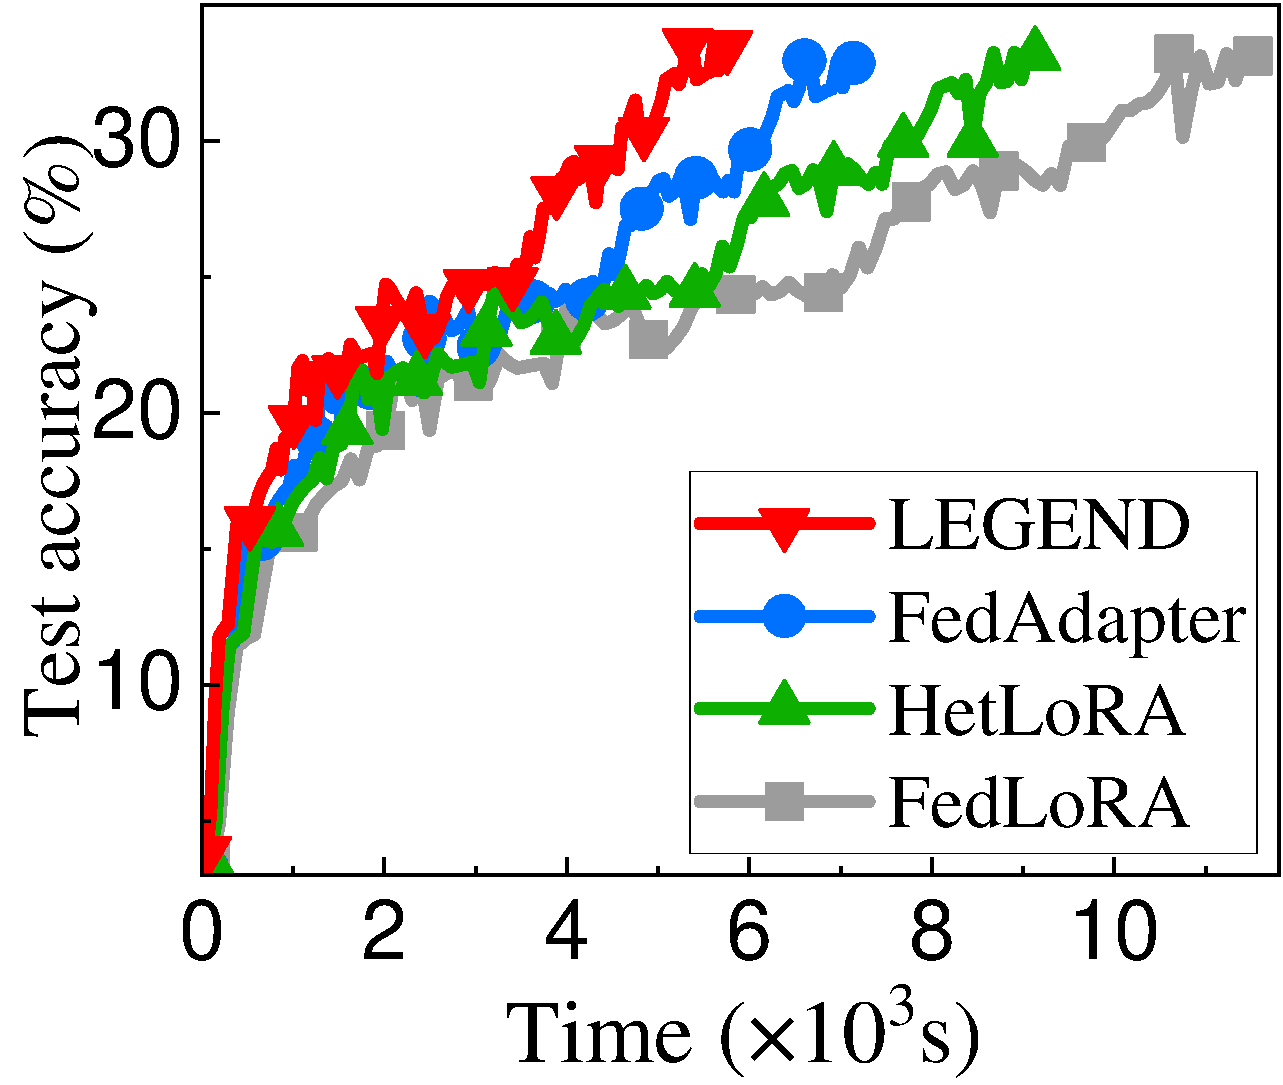
\includegraphics[width=1.57in]{figs/llama2-7b-gsm8k.pdf}
        \end{minipage}%
        \label{llama2-7b-gsm8k-time2acc}
    }%
    \subfigure[Time to reach 30\% accuracy]{
        \begin{minipage}[b]{0.5\linewidth}
        \centering
        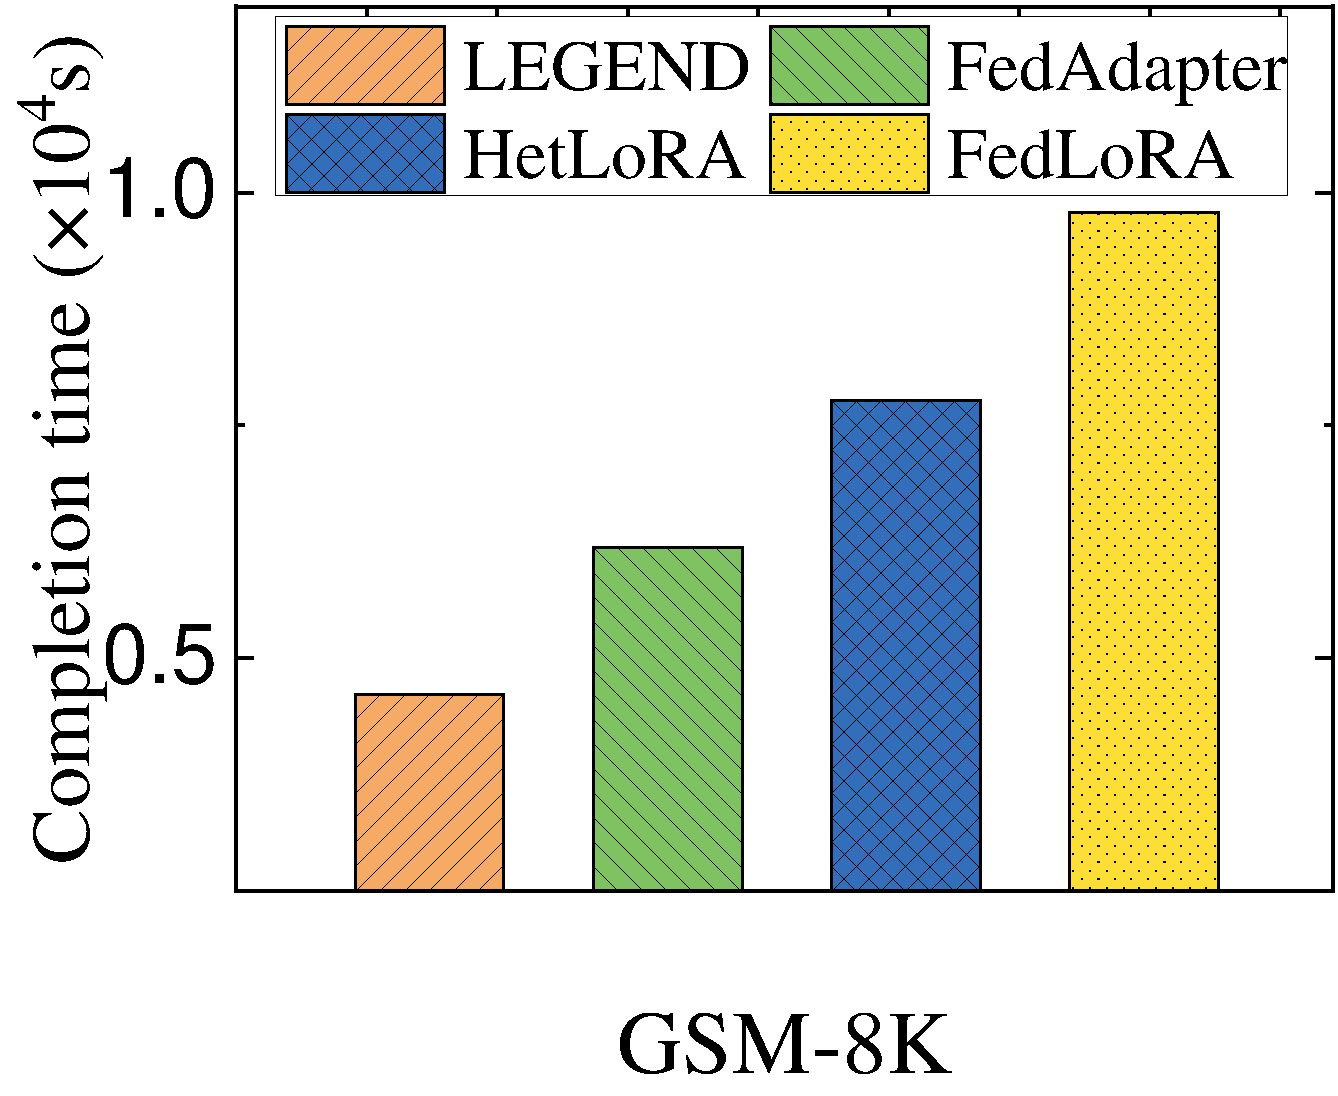
\includegraphics[width=1.6in]{figs/completion-time-gsm8k.pdf}
        \end{minipage}%
        \label{llama2-7b-gsm8k-completion}
    }%
    \centering
    \vspace{-0.3cm}
    \caption{\bluenote{Results on mathematical reasoning tasks.}}
    \label{gsm8k-results}
    \vspace{-0.5cm}
\end{figure}

\begin{figure*}
	\centering
	\subfigure[Traffic to reach 95\% accuracy]{
		\begin{minipage}[b]{0.23\textwidth}
			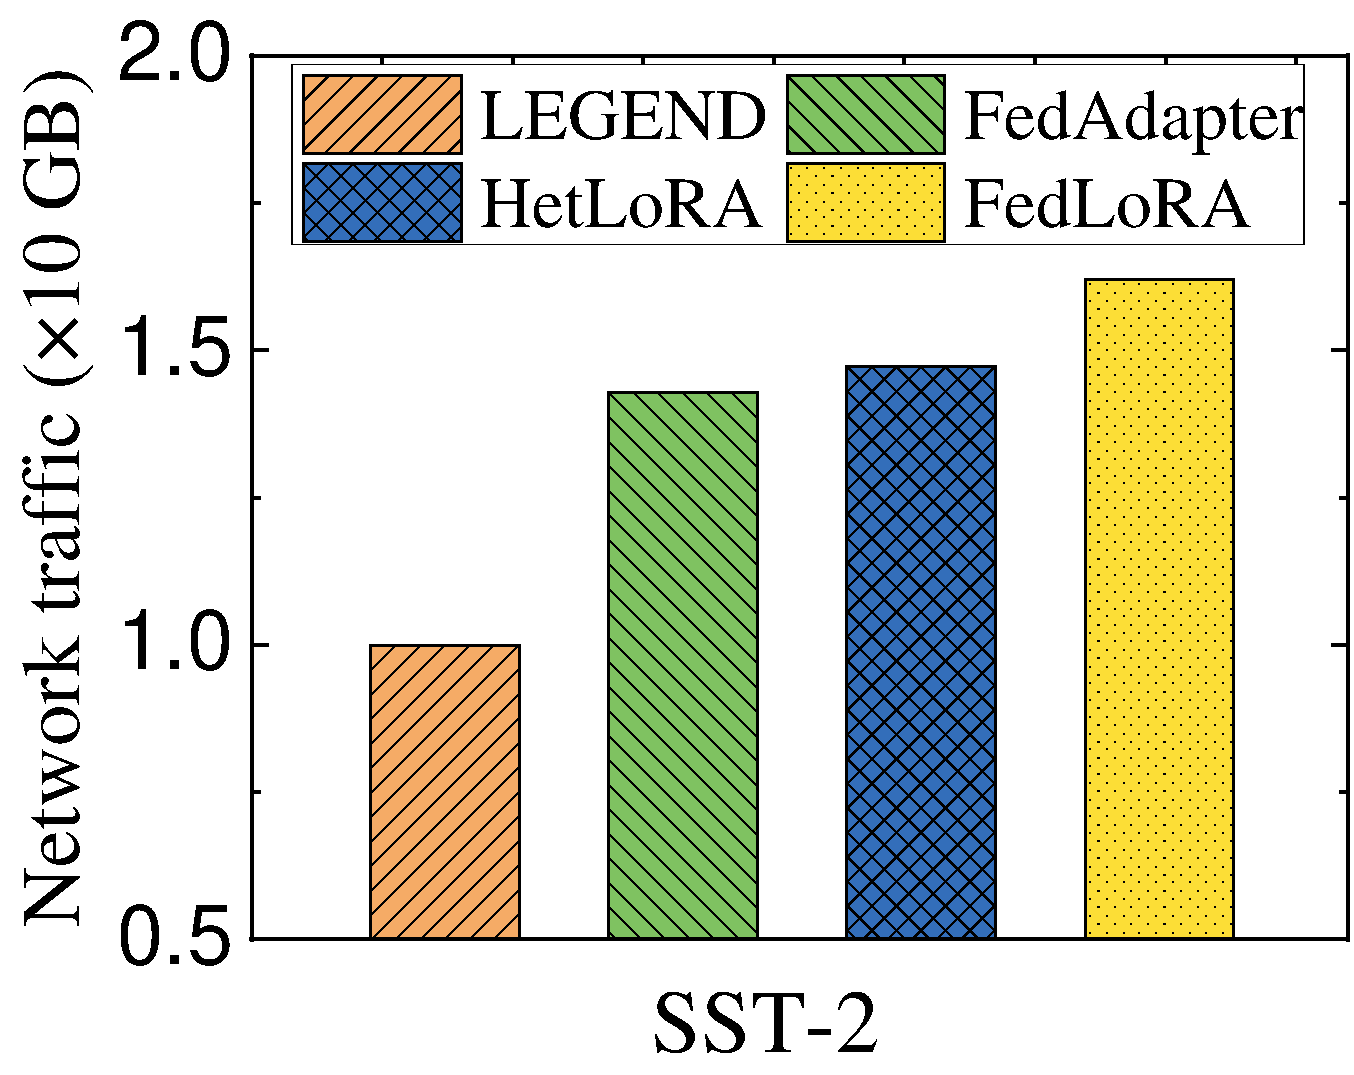
\includegraphics[width=1\textwidth]{figs/network-traffic-sst2.pdf} 
		\end{minipage}
		\label{roberta-traffic-sst2}
	}
    	\subfigure[Traffic to reach 90\% accuracy]{
    		\begin{minipage}[b]{0.23\textwidth}
   		 	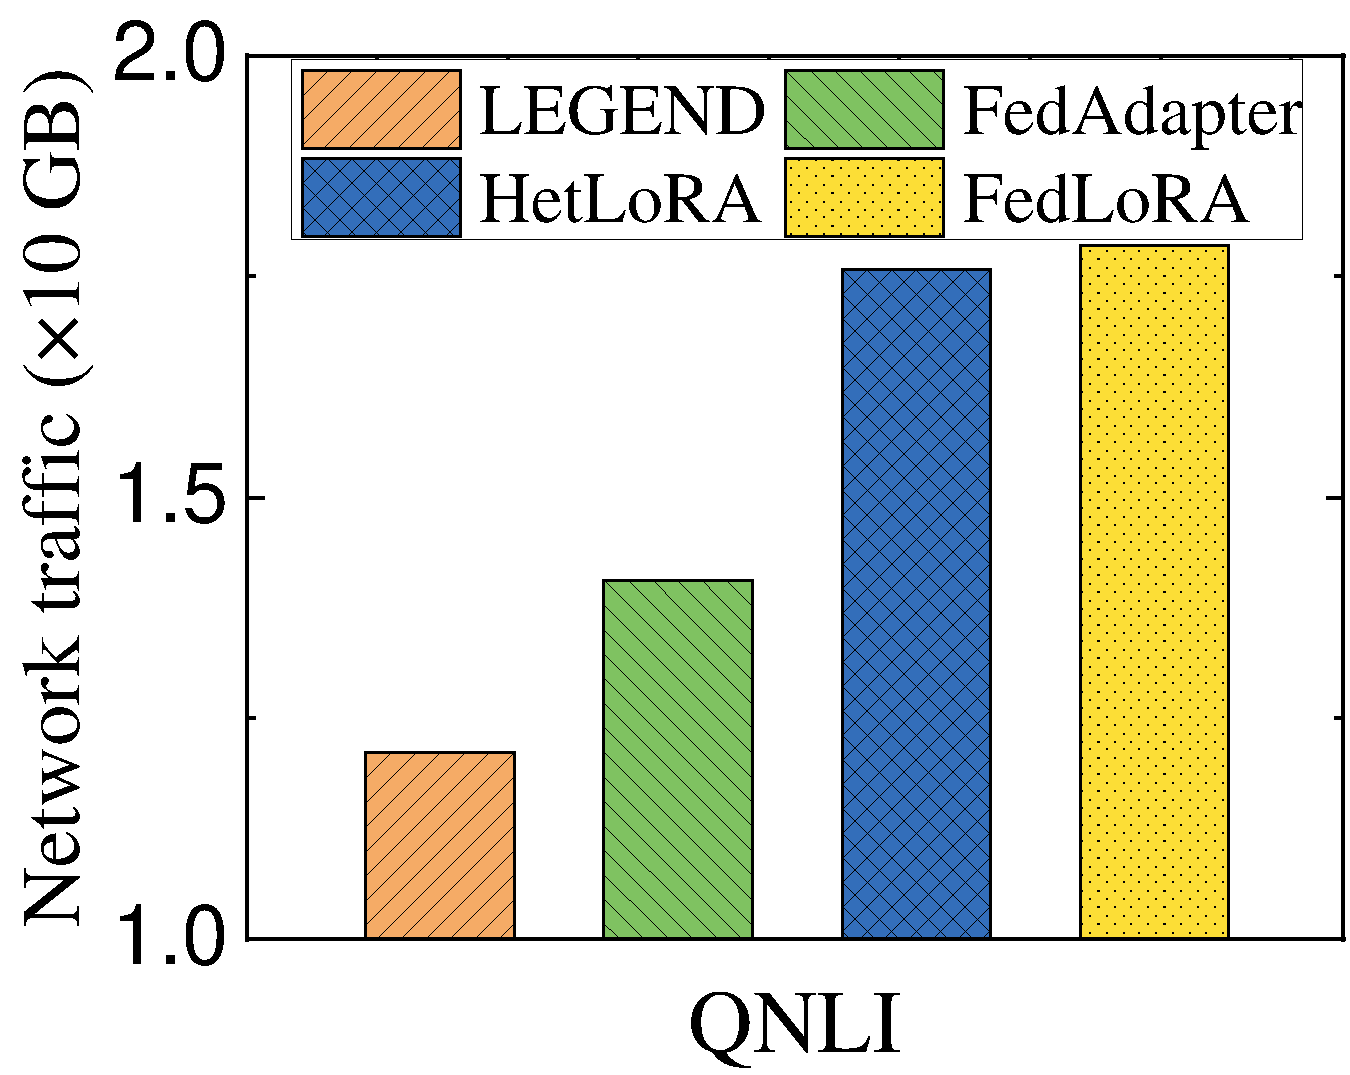
\includegraphics[width=1\textwidth]{figs/network-traffic-qnli.pdf}
    		\end{minipage}
		\label{roberta-traffic-qnli}
    	}
	% \\ 
	\subfigure[Traffic to reach 87\% accuracy]{
		\begin{minipage}[b]{0.23\textwidth}
			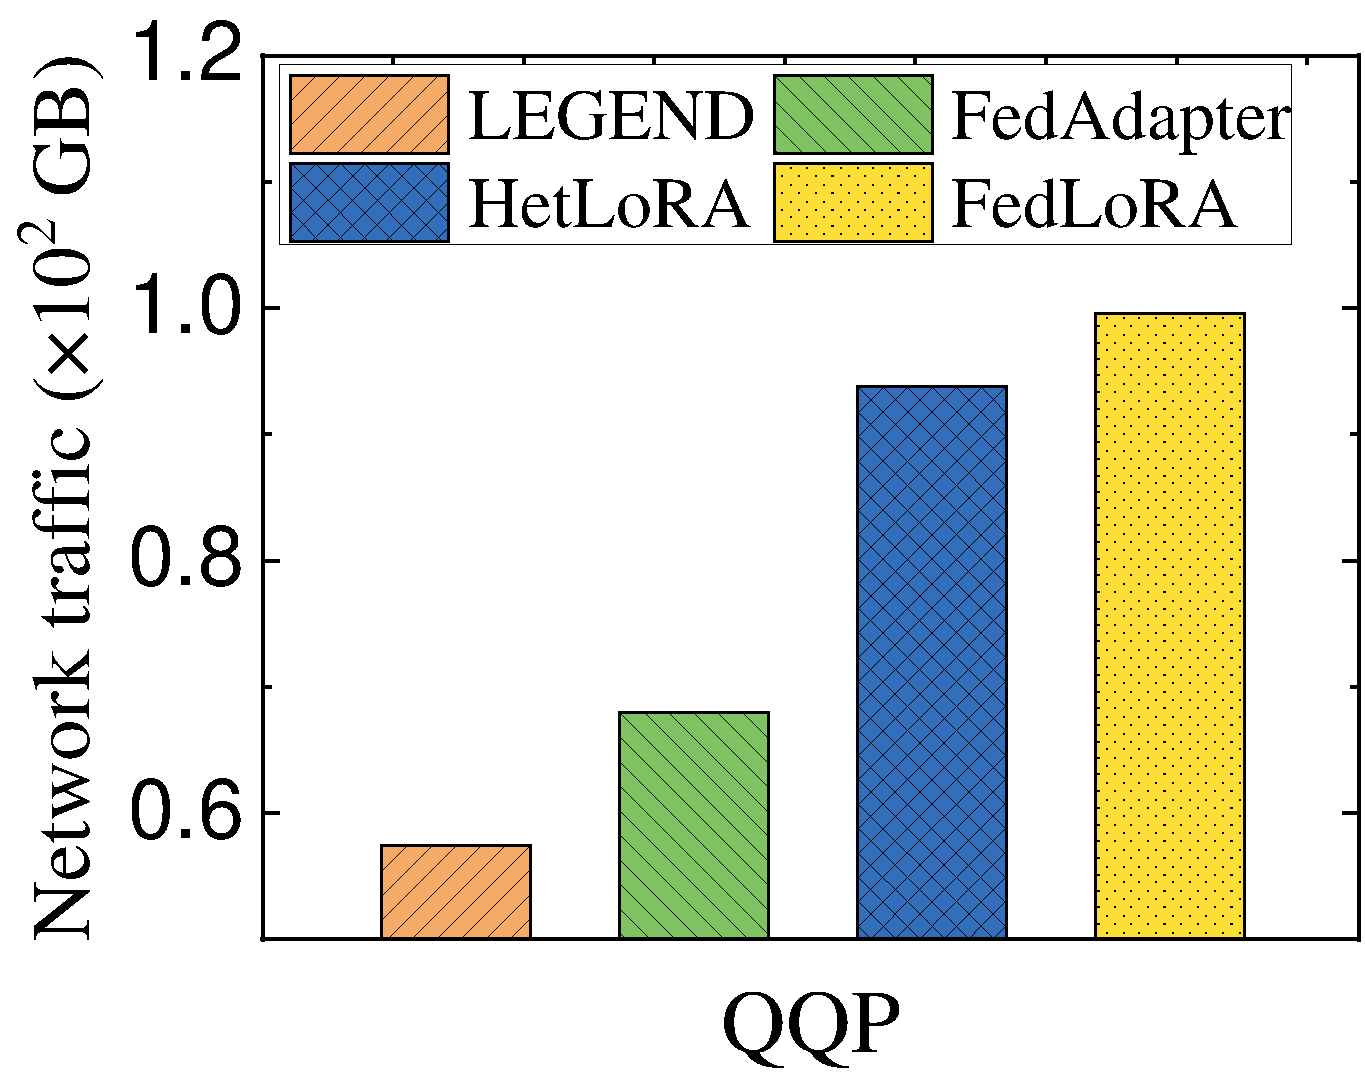
\includegraphics[width=1\textwidth]{figs/network-traffic-qqp.pdf} 
		\end{minipage}
		\label{deberta-traffic-qqp}
	}
    	\subfigure[Traffic to reach 85\% accuracy]{
    		\begin{minipage}[b]{0.23\textwidth}
		 	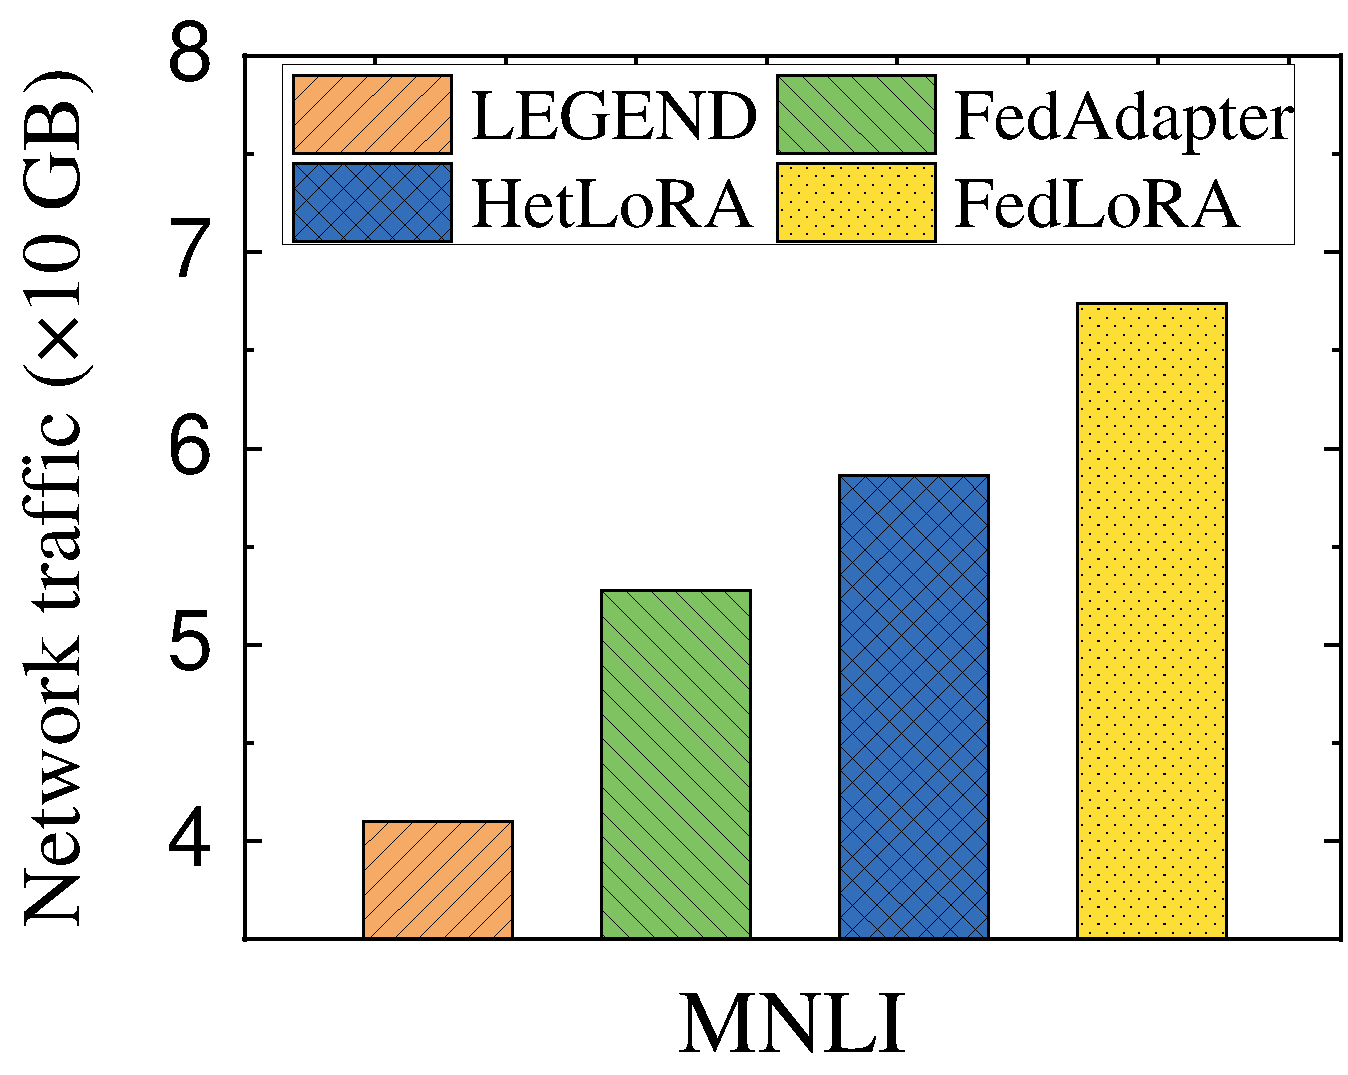
\includegraphics[width=1\textwidth]{figs/network-traffic-mnli.pdf}
    		\end{minipage}
		\label{deberta-traffic-mnli}
    	}
        \vspace{-0.3cm}
	\caption{Communication traffic of four approaches on general language understanding tasks.}
	\label{network-traffic}
        \vspace{-0.4cm}
\end{figure*}
\begin{figure*}
	\centering
	\subfigure[SST-2]{
		\begin{minipage}[b]{0.23\textwidth}
			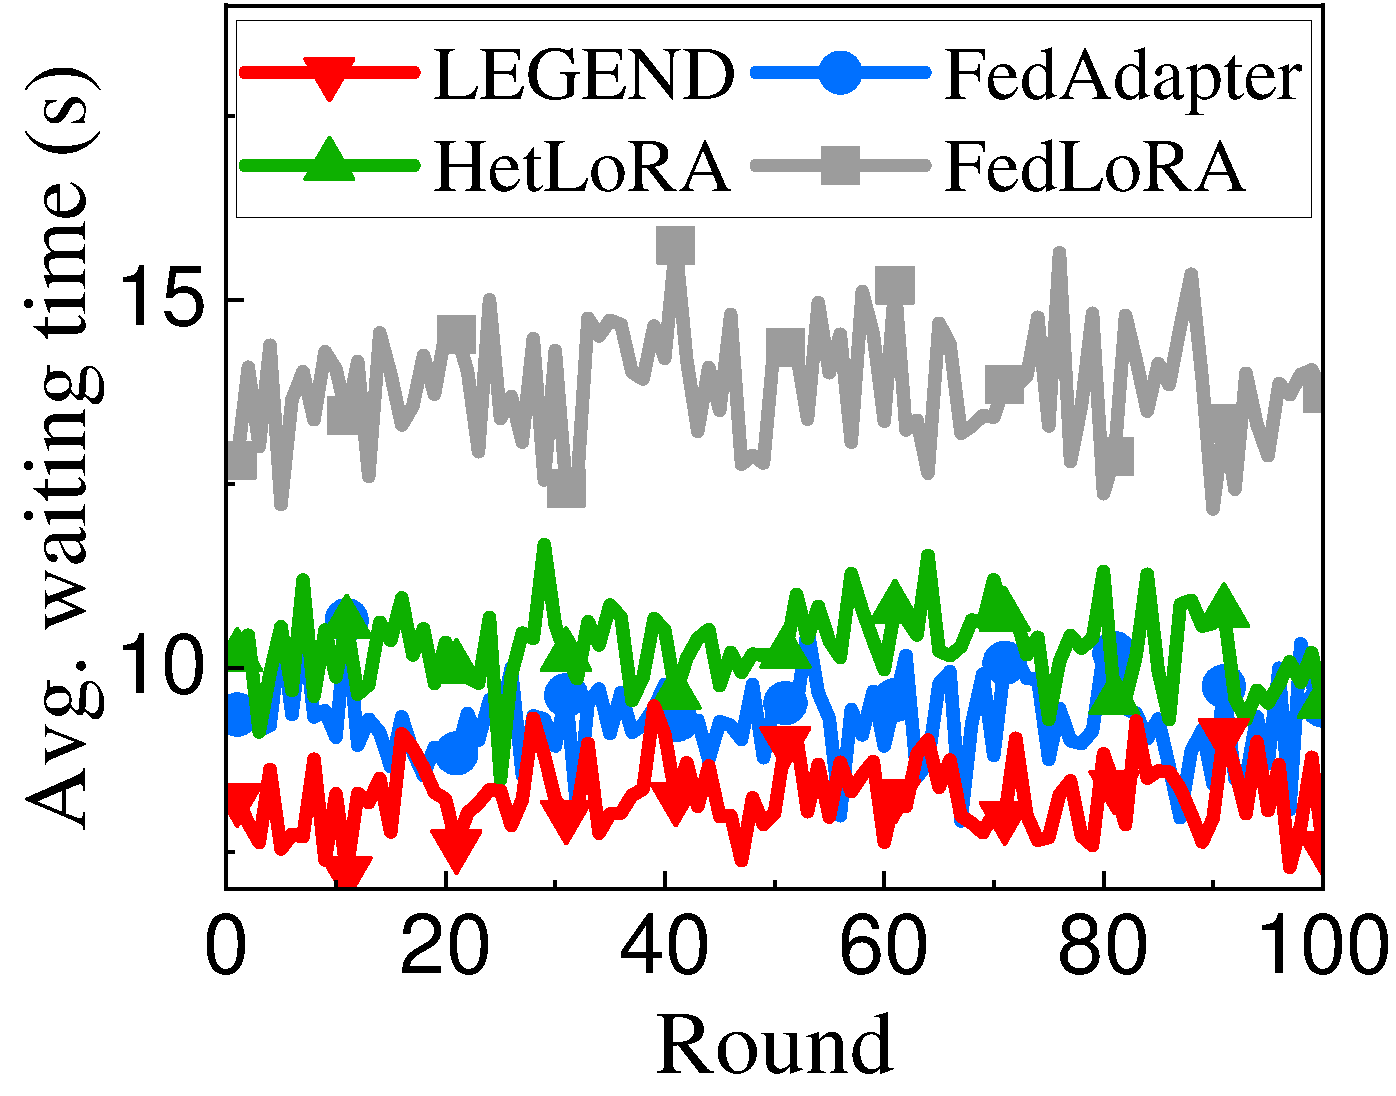
\includegraphics[width=1\textwidth]{figs/final-waiting-time-sst2.pdf} 
		\end{minipage}
		\label{roberta-waiting-sst2}
	}
    	\subfigure[QNLI]{
    		\begin{minipage}[b]{0.23\textwidth}
   		 	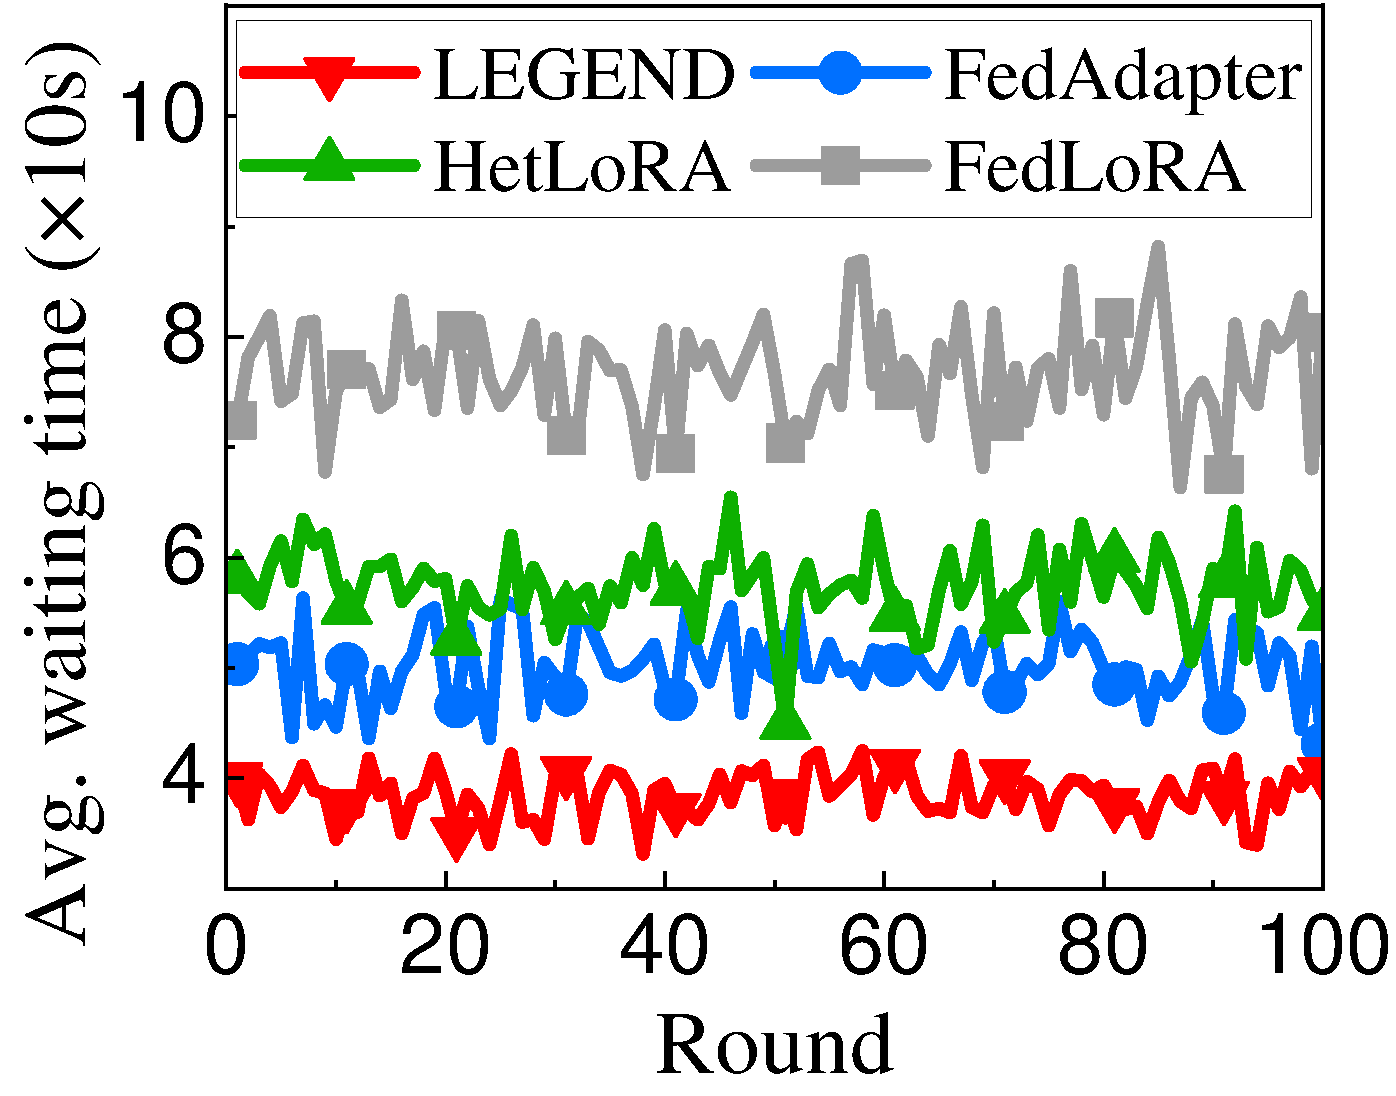
\includegraphics[width=1\textwidth]{figs/final-waiting-time-qnli.pdf}
    		\end{minipage}
		\label{roberta-waiting-qnli}
    	}
	% \\ 
	\subfigure[QQP]{
		\begin{minipage}[b]{0.23\textwidth}
			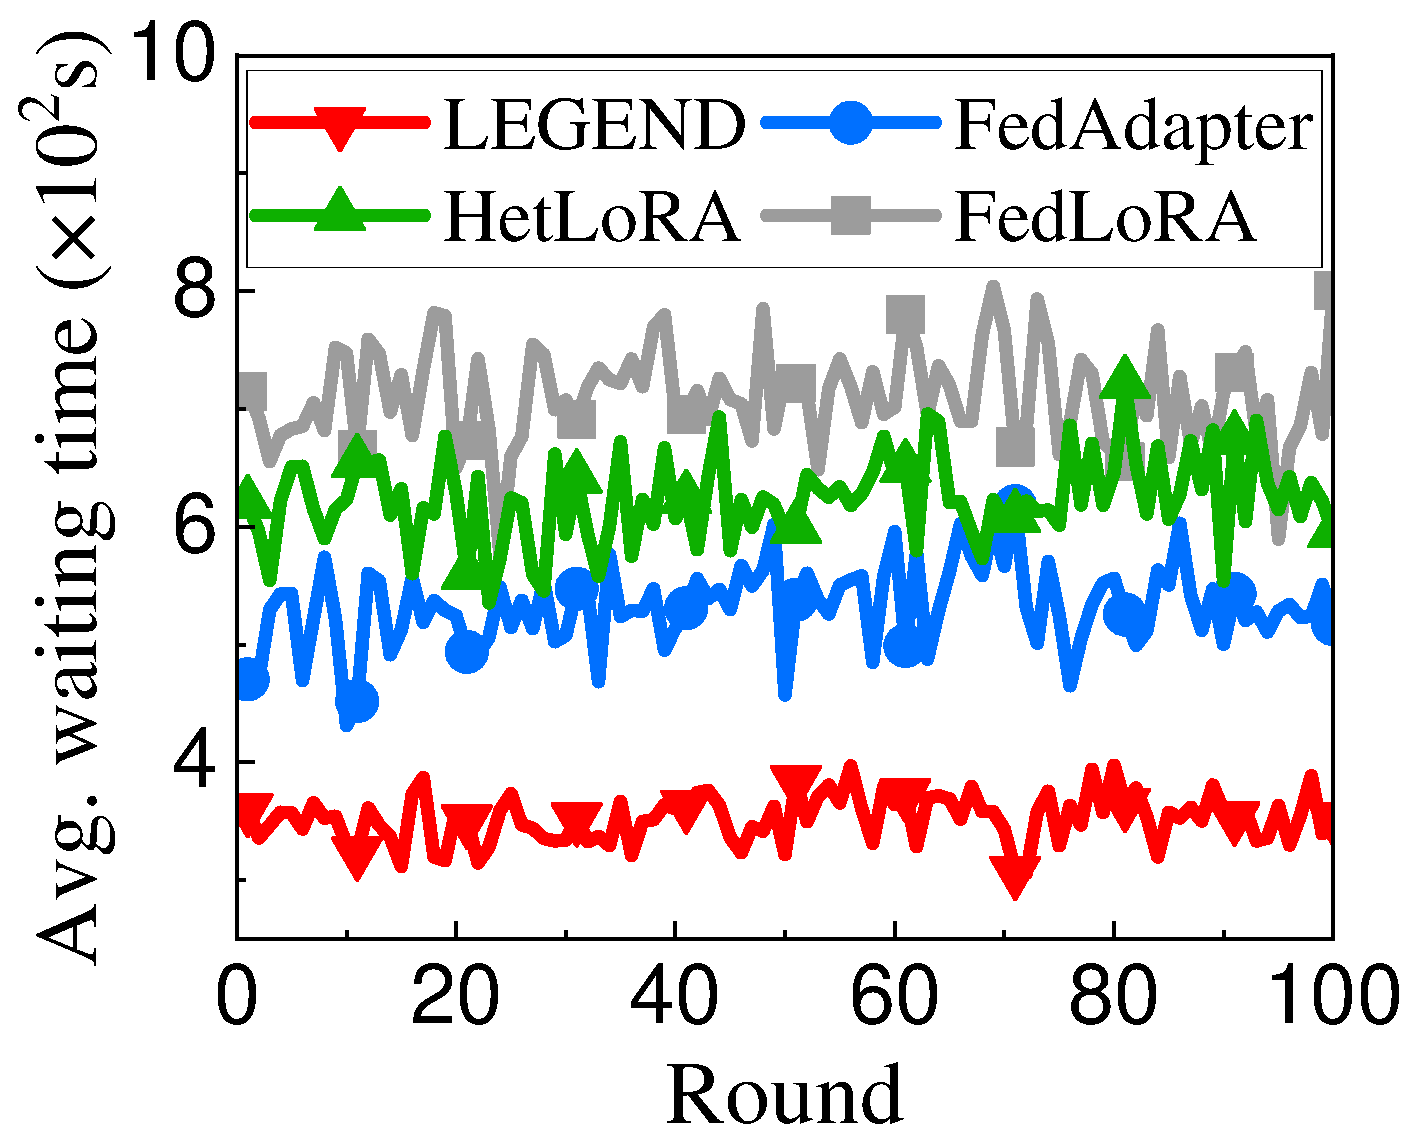
\includegraphics[width=1\textwidth]{figs/final-waiting-time-qqp.pdf} 
		\end{minipage}
		\label{deberta-waiting-qqp}
	}
    	\subfigure[MNLI]{
    		\begin{minipage}[b]{0.23\textwidth}
		 	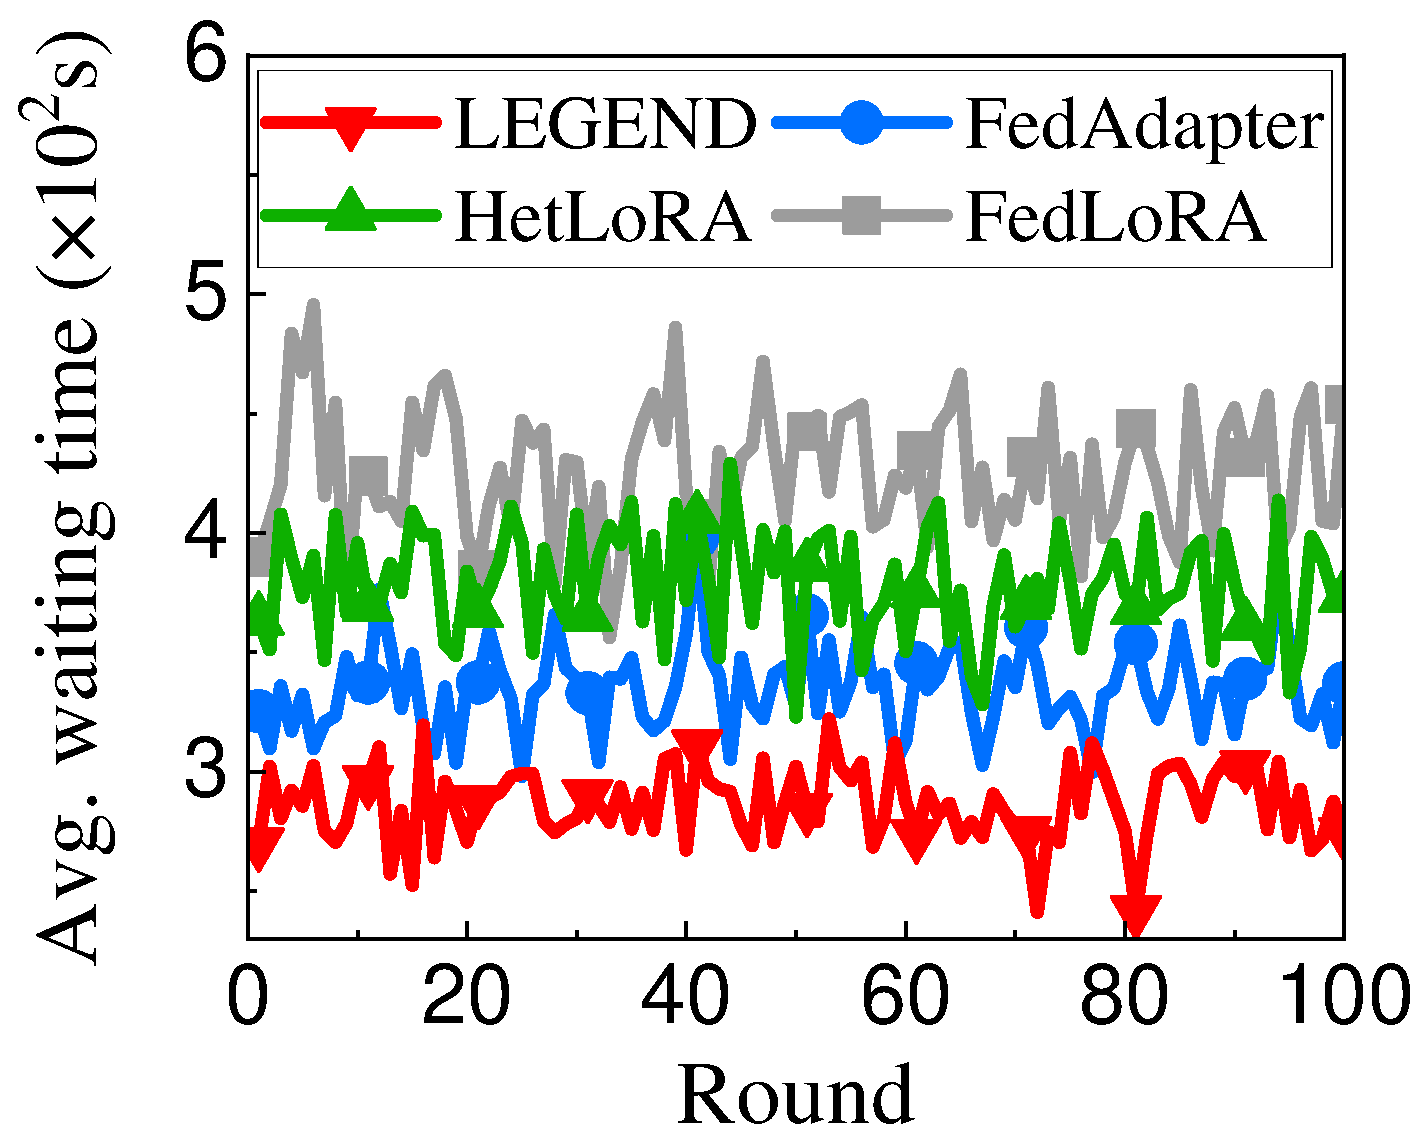
\includegraphics[width=1\textwidth]{figs/final-waiting-time-mnli.pdf}
    		\end{minipage}
		\label{deberta-waiting-mnli}
    	}
        \vspace{-0.3cm}
	\caption{Average waiting time of four approaches on general language understanding tasks.}
        \label{average-waiting-time}
        \vspace{-0.4cm}
\end{figure*}
% \textbf{Reducing communication cost.}
% \textbf{Communication Cost.}
Secondly, to illustrate the advantage of LEGEND in saving communication resources, we evaluate the communication traffic consumption of these approaches when achieving the target accuracy.
According to the results in Figure \ref{network-traffic}, LEGEND always causes the least communication traffic among all approaches. 
For example, as shown in Figure \ref{roberta-traffic-sst2}, when achieving 95\% accuracy, LEGEND consumes 9.9GB, while FedAdapter, HetLoRA, and FedLoRA consume 14.2GB, 14.7GB, and 16.2GB, respectively.
Compared with FedAdapter, HetLoRA, and FedLoRA, LEGEND reduces communication traffic by about 30.0\%, 32.1\%, and 38.3\%, respectively.
On one hand, compared to FedLoRA and HetLoRA which add LoRA layers of the same rank to all layers, LEGEND generates adaptive LoRA depth and rank distribution to accommodate heterogeneous devices. 
On the other hand, unlike FedAdapter which requires multiple device groups to find the optimal adapter structure, LEGEND determines the suitable LoRA configuration based on the device's status, making fine-tuning more efficient and thus reducing communication overhead.
Besides, by Figure \ref{roberta-traffic-qnli}, LEGEND consumes 12.1GB when achieving 90\% accuracy for QNLI, reducing the communication traffic by about 1.95GB, 5.46GB, and 5.74GB  compared with FedAdapter, HetLoRA, and FedLoRA, respectively.
For QQP, the results in Figure \ref{deberta-traffic-qqp} show that LEGEND reduces the total traffic consumption up to 42.3\% when achieving accuracy. 
Moreover, by Figure \ref{deberta-traffic-mnli}, when achieving 85\% accuracy for MNLI, LEGEND consumes 42GB, while FedAdapter, HetLoRA, and FedLoRA consume about 54GB, 60GB, and 69GB, respectively. 
\bluenote{
% By dynamically adapting LoRA depths to accommodate heterogeneous devices, LEGEND enables each device to transmit only its corresponding LoRA layers, thereby significantly reducing communication overhead.
The experimental results underscore the advantages of LEGEND in reducing communication costs. 
}
% This is because LEGEND distributes fewer parameters to resource-constrained devices, saving a lot of communication resources compared to other methods of delivering the same parameters to all devices.
% These results demonstrate the communication efficiency of LEGEND. 



% \textbf{Mitigating System Heterogeneity.}
To demonstrate the effectiveness of LEGEND towards system heterogeneity, we illustrate the average waiting time of the four approaches on the four datasets in Figure \ref{average-waiting-time}.
\bluenote{
LEGEND achieves the shortest waiting time across all datasets by assigning different LoRA depths with reasonable rank distribution to heterogeneous devices.
}
% On the contrary, HetLoRA and FedLoRA injected LoRA layer to all transformer layers in the LM, leading to prolonged fine-tuning time on resource-constrained devices, while FedAdapter speeds up the training process by picking the best training group in each round.
% For example, by Figure \ref{roberta-waiting-sst2}, the average waiting time of LEGEND is 8.3s for SST-2, while FedAdapter, HetLoRA, and FedLoRA incur average waiting time of 9.3s, 10.2s, and 13.8s, respectively.
% Compared with FedAdapter, HetLoRA, and FedLoRA, LEGEND separately improves the average waiting time by about 11.0\%, 19.5\%, and 40.2\%.
For example, by Figure \ref{roberta-waiting-sst2}, LEGEND separately improves the average waiting time by about 11.0\%, 19.5\%, and 40.2\%, compared with FedAdapter, HetLoRA, and FedLoRA for SST-2.
By Figure \ref{roberta-waiting-qnli}, the average waiting time of LEGEND is 38.6s for QNLI, while FedAdapter, HetLoRA, and FedLoRA incur average waiting time of 50.3s, 57.4s, and 76.7s, respectively.
LEGEND reduces the average waiting time by about 23.4\%, 32.8\%, and 49.7\% compared to FedAdapter, HetLoRA, and FedLoRA, respectively.
Besides, as illustrated by Figure \ref{deberta-waiting-qqp}, the average waiting time of LEGEND is 352s for SST-2 while FedAdapter, HetLoRA, and FedLoRA incur an average waiting time of 532s, 623s, and 710s, respectively.
Compared with FedAdapter, HetLoRA, and FedLoRA, LEGEND reduces the average waiting time by about 33.8\%, 43.5\%, and 50.4\%, respectively.
In addition, by Figure \ref{deberta-waiting-mnli}, LEGEND also outperforms FedAdapter, HetLoRA, and FedLoRA, reducing the averaging waiting time by 14\%, 24\%, and 32.7\%, respectively.
LEGEND achieves the least waiting time across all tasks by assigning appropriate depth to devices, significantly reducing the time for local fine-tuning on resource-constrained devices.
In contrast, FedLoRA adds LoRA layers to all transformer layers of the model, which requires the complete backpropagation process to update all LoRA layers and fast devices should be forced to wait for slow ones, leading to prolonged waiting time and poor fine-tuning efficiency.
HetLoRA improves FedLoRA by assigning diverse ranks to the devices to alleviate the challenge of system heterogeneity but with limited success, while FedAdapter speeds up the fine-tuning process by selecting the best fine-tuning group from groups with different Adapter configurations in each round.
These experimental results demonstrate the superiority of LEGEND in mitigating system heterogeneity.
\vspace{-0.3cm}
% \textbf{Performance on Decoder-only Models.} 
% \bluenote{
% Secondly, we conduct sets of experiments with decoder-only models (\ie, Llama2-7B \cite{touvron2023llama}) to evaluate the performance of the four approaches. 
% The experimental results are presented in Figures \ref{mmlu-results} and \ref{gsm8k-results}.
% LEGEND greatly outperforms other approaches by a significant margin when fine-tuning Llama2-7B on MMLU and GSM-8K.

% }




\vspace{-0.1cm}
\subsection{Ablation Study}
\vspace{-0.1cm}
\label{sec-ablation}
% \textbf{The impact of rank distribution under different budget?}
% \textbf{\rednote{The impact of $\lambda$}}
There are two key factors in LEGEND, \ie, LoRA depth and rank distribution, which are developed to enhance the performance of FedLoRA.
Herein, we conduct several sets of ablation experiments on SST-2 and QNLI to validate the effectiveness of the two essential factors. 
We adopt LEGEND, LEGEND without LoRA depth (denoted as LEGEND w/o LD), LEGEND without rank distribution (denoted as LEGEND w/o RD) as the baselines.
% Specifically, in LEGEND w/o LD, the PS directly generates an gradually increasing rank distribution, but all devices have the same LoRA depth as FedLoRA, while in LEGEND w/o RD, all devices are assigned adaptive LoRA depths, but the ranks across different layers of the model are the same.
As illustrated in Figure \ref{ablation}, both LoRA depth and rank distribution are essential in LEGEND, but they contribute to the system in different ways.
\bluenote{
% Specifically, LoRA depth affects completion time, while rank distribution significantly influences final fine-tuning performance.
For instance, by Figures \ref{ablation-rank-time2acc-sst2} and \ref{ablation-rank-time2acc-qnli}, LEGEND w/o LD achieves similar final test accuracy, \eg, 95.3\% on SST-2 and 91.6\% on QNLI, compared with LEGEND, while LEGEND w/o RD slightly degrades to 94.6\% on SST-2 and 90.5\% on QNLI, respectively.
Besides, by Figure \ref{ablation-rank-time2acc-sst2}, when achieving a target accuracy of 94\% on SST-2, LEGEND saves the completion time by about 50.3\% and 54.5\% compared with LEGEND w/o RD and LEGEND w/o LD, respectively.
By Figure \ref{ablation-rank-time2acc-qnli}, compared with LEGEND w/o RD and LEGEND w/o LD, LEGEND separately speeds up fine-tuning by about 1.38$\times$ and 1.93$\times$, when achieving the same target accuracy (\ie, 90\% on QNLI). 
On the one hand, by employing a reasonable rank distribution and enabling all devices to fine-tune all LoRA layers, LEGEND w/o LD enhances the fine-tuning performance, but results in prolonged waiting time and slow convergence rates. 
On the other hand, LEGEND w/o RD assigns adaptive LoRA depth for the devices with uniform ranks across all layers, failing to strategically allocate larger rank to critical layers (\eg, deep layers), which constrains the fine-tuning performance and leads to performance degradation.
The results demonstrate the positive roles of the two designs.
}
\vspace{-0.2cm}


% \vspace{-0.2cm}

% \begin{table}
% \renewcommand{\arraystretch}{1.1}
%     \centering
%     \caption{\rednote{Ablation study of rank distribution under different depth}}
%     % \vspace{-5px}
%     \resizebox{\linewidth}{!}{
%     \begin{tabular}{cccc}
%         \Xhline{1pt}
%         \makecell[l]{\textbf{LoRA depth}} & \textbf{Methods} & \textbf{Completion Time} & \textbf{Traffic} 
%         \\\Xhline{0.7pt}
%         % $\beta=0.0$ & Few-shot CoT & NA & 13.42\% (177/1319) \\\hdashline
%         \multirow{4}{*}{12} & FedLoRA &  &   \\
%         & HetLoRA &  &  \\
%         &  FedAdapter &  &  \\
%         &  LEGEND &  & \\ \Xhline{0.7pt}
%         \multirow{4}{*}{8} & FedLoRA & &   \\
%         & HetLoRA & &  \\
%         &  FedAdapter &  &  \\
%         &  LEGEND &  &  \\ \Xhline{0.7pt}
%         \multirow{4}{*}{4} & FedLoRA &  &   \\
%         & HetLoRA &  &  \\
%         &  FedAdapter &  &  \\
%         &  LEGEND &  &  \\ 
%         \Xhline{1pt}
%     \end{tabular}
%     }
%     \label{tab:gsm8k}
%     % \vspace{-10px}
% \end{table}

% \begin{figure}[t]
%     \centering
%     \subfigure[Test accuracy]{
%         \begin{minipage}[t]{0.5\linewidth}
%         \centering
%         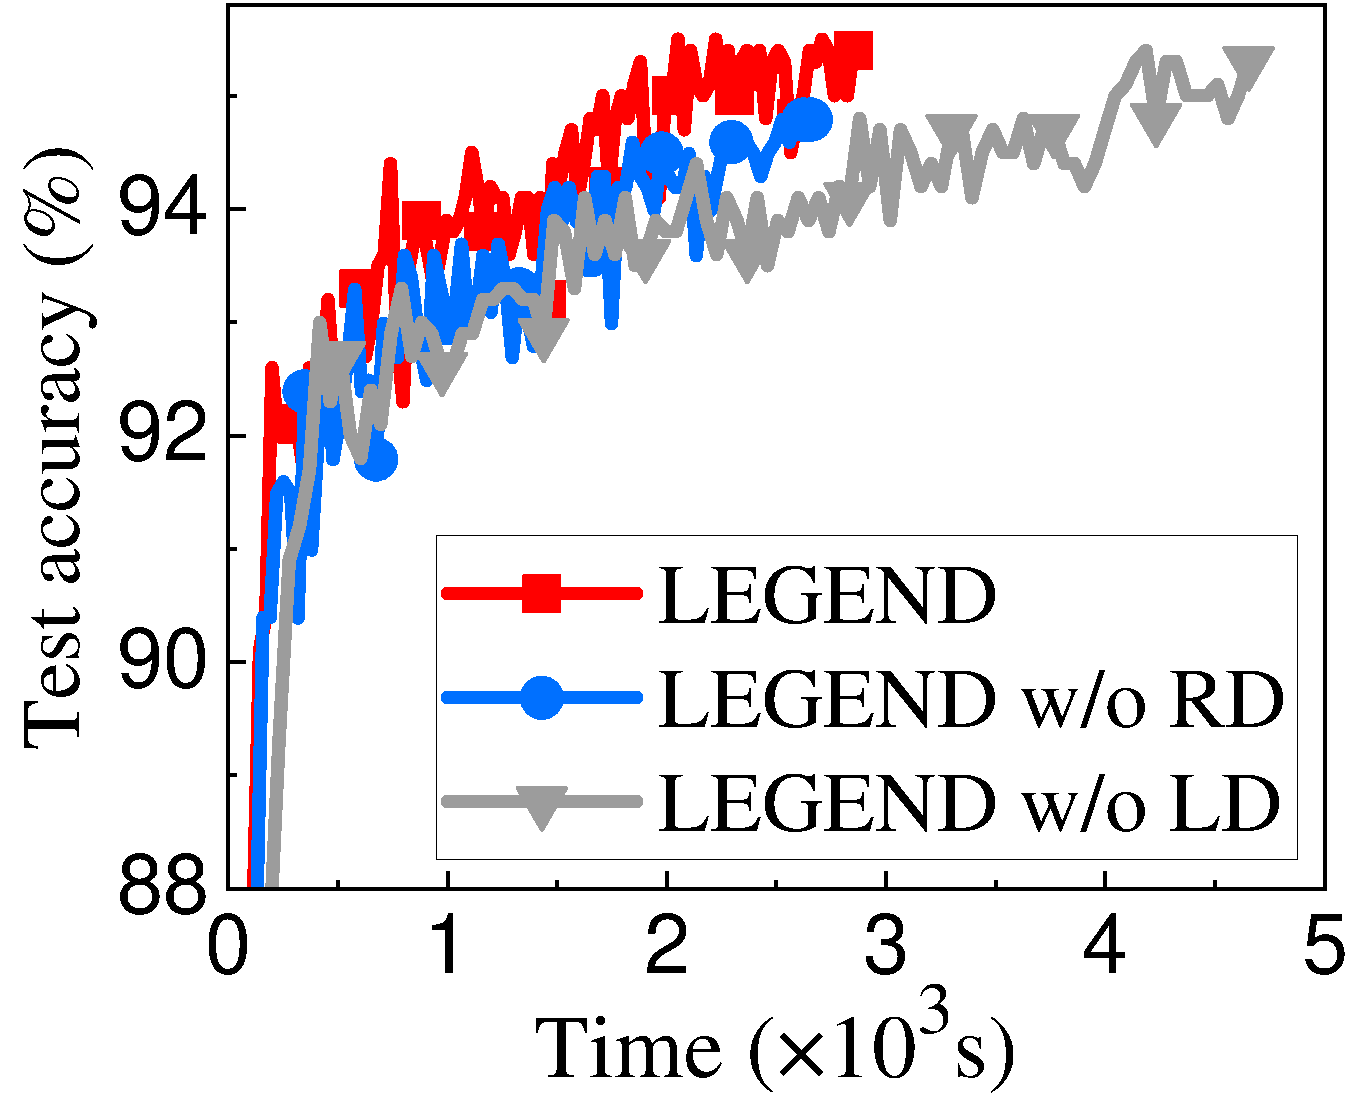
\includegraphics[width=1.5in]{figs/ablation-module-sst2-time2acc.pdf}
%         \end{minipage}%
%         \label{ablation-rank-time2acc-sst2}
%     }%
%     \subfigure[Time to reach 95\% accuracy]{
%         \begin{minipage}[t]{0.5\linewidth}
%         \centering
%         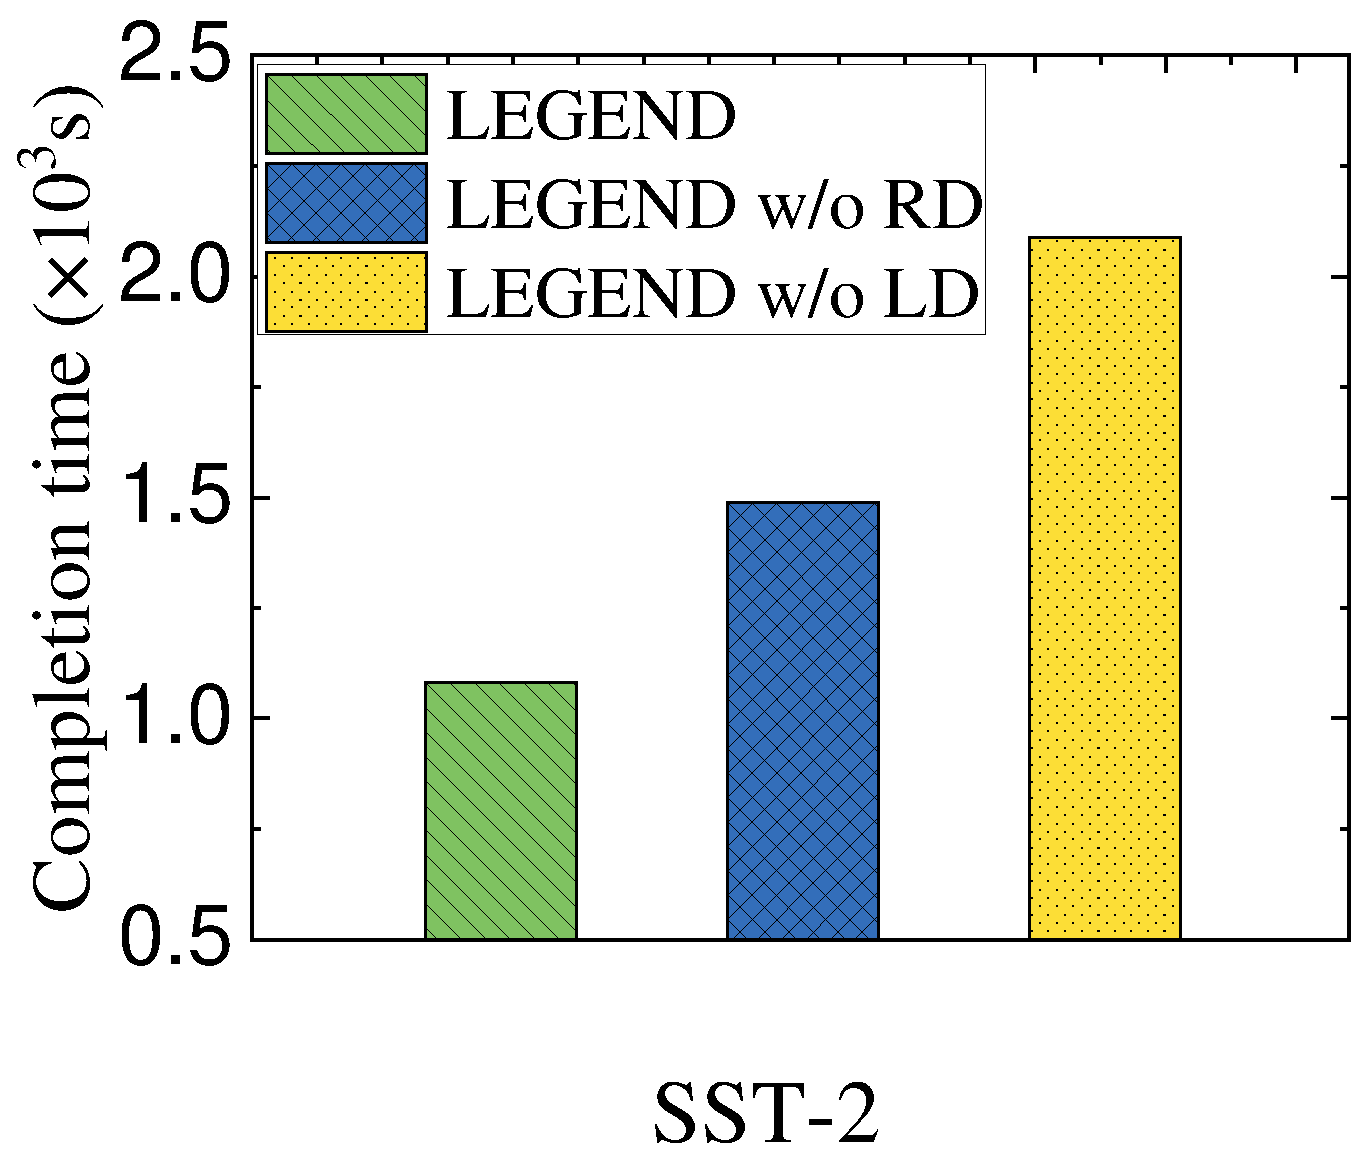
\includegraphics[width=1.5in]{figs/ablation-module-sst2-completion-time.pdf}
%         \end{minipage}%
%         \label{ablation-rank-completion-sst2}
%     }%
%     \centering
%     \vspace{-0.25cm}
%     \caption{\rednote{Ablation study of rank distribution on SST-2}.}
%     \label{ablation-module-sst2}
%     \vspace{-0.5cm}
% \end{figure}

% \subsection{\rednote{Effect of System Scales}}
% \rednote{
% Simulation
% 100 - 1000
% }
